%===============================================================================
%          File: ch3_machine_learning.tex
%        Author: Pedro Ferrari
%       Created: 08 Feb 2017
% Last Modified: 08 Feb 2017
%   Description: Chapter 3: Machine Learning
%===============================================================================
\chapter{Machine Learning}
\label{cha:machine_learning}


\section{Preamble}\label{section-preamble}
Most of the discussions in this chapter are based on information extracted from two distinguished textbooks: \ref{bishop-patternRecognition} and  \ref{hastie-elemstatslearn}. Some fundamental concepts and material were also used from \label{scikit-learn}. While other texts were also used, it is not necessary that we point them out here as they have been correctly cited. Where not specified, the reader can assume that the proof is based from said texts.


\section{ Brief ovierview to machine learning and supervised classification problems}\label{section-introduction}

Machine learning is a subfield of computer science with broad \textit{theoeretical} intersections with statistics and mathematical optimization. At present time it has a wide range of applications. A non-comprehensive list of its use includes self-driving cars, spam detection systems, face and/or voice recognition, temperature prediction in weather, AI opponents in games, disease prediction in patients, text and audio language translation, stock pricing, movie recommendation systems, etc. Examples of these machine learning programs are now widespread to the point where their use today has direct impact on the lives of millions of people. Due to this, machine learning has \textit{practical} intersections with data and software engineering.

The most widely used definition of machine learning is attributed to Tom Mitchell:
"A computer program is said to learn from experience E with respect to some class of tasks T and performance measure P if its performance at tasks in T, as measured by P, improves with experience E" \textcite{Mitchell-MLearning}. To our purpose it is clear though that this definition \footnote{Other authors might reference machine learning as \textit{statistical learning}. See \textcite{hastie-elemstatslearn} as an example.} is not formally well-defined. However it serves to convey the idea of algorithms that automatically \textit{learn} to do a a specific task better over time and with more data. Note that the "goodness" of their performance is inherently subjected to the evaluation criteria chosen for the task. Because of this,\textit{learning} is less associated with a cognitive definition in this context and more to a performance based approach.

Machine Learning is divided into two main categories: Supervised and Unsupervised Learning. Let $Y \in \mathbb{R}^n$ be the outputs of the model and $X \in \mathbb{R}^{n \times  p}$ be the inputs: for supervised learning algorithms are set to produce outputs from input data i.e. for each instance $n$, the computer has access to examples of outputs and tries to reproduce them based on information contained in $X$. In this context, the algorithm is generally referred to as a \textit{learner}.

The second class of problems is where the output $Y$ is missing altogether from the data. In this scenario the most common objectives are clustering samples, density estimation and data compression. Linear regression and K-means clustering are examples of algorithms in each of these categories respectively.

In supervised learning tasks can be sub-categorized by the nature of the problem. When the type of the output variable $Y$ takes a (generally \textit{small} )discrete set of values then it is said that it is a supervised \textit{classification} problem. On the other hand, when the output takes continuous (or dense in an open set of $\mathbb{R}$) range of \textit{quantitative} values, the problem is said to be of supervised \textit{regression}. Note that regression problems can be encoded into classification problems by grouping the output values into categories by taking ranges of output values.

Suppose our objective is to predict $y$ given a new sample $x$. In supervised regression problems, $y$ will comprise a continuous variable. for classification problems on the other hand, $y$ will represent a label for a certain class. For the case of $K$ classes, $y$ most commonly takes values in the ranges $0$ through $K-1$  or $1$ through $K$. In both cases, the joint probability distribution $p(X, Y)$, called the \textit{true} distribution, gives all of the information we need on these two variables. However the values of this probability is most often unknown. The idea is to then user estimations and inference on the most likely values for new samples and take decisions with the information at hand. These decisions will be based on the most probabilistic characterization of the data we have. In this work we will focus on the classification aspect of machine learning.

In these type of problems the theoretical and the computational aspects are both of interest. The algorithms used need to consider the technical requirements of the software and hardware at hand, as well as the time or resource constrains imposed by the problem setting. As such, they are expected to be executed in a reasonable amount of time, imposed by the task specification, and limited by the computing power available. \footnote{Here the word \textit{reasonable} is used in a broad sense. It will depend entirely on time constraints, computational capacity, usage and other aspects of each learning application.} There can be  problems which require that the algorithm output predictions in \textit{real-time}, to the resolution of milliseconds. Picture a system where a credit-card transaction needs to be approved or labeled as fraud. Here the system needs to respond in short time if the transaction is fraudulent.

Other use cases might require the system to process a big volume of data at once, not a single event, but a batch of these and output this answer. The system in use needs to be prepared to run \textit{lean} with a big inflow of data, without overloading the hardware capacity.  These examples show that for a given problem, multiple algorithms are available to use but while all of them are theoretically doing the same task, we must also consider the practical advantages of these. Computational efficiency and \textit{scalability} are relevant when working with these problems. Even though we won't delve into these aspects in this work, it has an important consideration in the application of Machine Learning solutions.


In its essence, a machine learning method is a probabilistic model built from data so it is very similar to a statistical model. However, it differs specially in that its focus is generally on the models' predictive abilities more than in the model's parameters estimates.\textcite{breiman-statisticalmodeling} The algorithms will be built and used to try and replicate as best as possible a given phenomena, without really identifying the true nature of the mechanisms behind this phenomena. As such, most applications will try to \textit{imitate} the task's behavior rather than try to identify the real system behind it.
%on this matter It also puts a great amount of weight on efficiency and computational scalability.

%At this point it is important to start noting

These subtle differences in the way machine learning approaches a problem is also reflected in the terminology used by the field. We know that different disciplines often speak about the same machine learning methods in different terms and this difference is most notable with classic statistics. Where we can, we will be identifying these differences along the text. As a start, the \textit{dependent} $Y$ is called the target or label and the \textit{independent} variables, \textit{covariates} or \textit{input variables} are named \textit{features} in this case.
%Labels that are representing categorical or discrete variables are also named factors or \textit{qualitative} variables.


\subsubsection{A working example}\label{section-example}

For the purpose of this work we will be talking of the training set, noted by $\mathrm{T}$ as the set of data examples. The objective is to build a probabilistic model which has the capacity to correctly predict the class instance of new data objects based on having seen information of other data objects.

For concreteness, let's consider a reduced dataset built from Call Detail Records (CDRs) where samples are calls being made by users who can belong to any of following provinces : \textit{Buenos Aires}, \textit{Cordoba} and \textit{Santa Fe}.
%\url{http://stackoverflow.com/}
%\footnote{For more information on this set, a historic review is given at \url{https://en.wikipedia.org/wiki/Iris_flower_data_set}}.
Five measurements were taken on all of the observations to account for the user's number of calls and total minute duration of calls during a week of measurements. A short overview of this dataset is printed below:

\begin{table}[ht]
\caption{{Head of the CDR dataset}}
\label{tab:sample_CDR}
\centering
\begin{tabular}{ l l l l l l }
\toprule
User & CallsWeekend & TimeWeekend & CallsWeekDays & TimeWeekday & Province \\
\midrule
BA343E  & 15 &  89 & 8 & 24 &  \textit{Santa Fe}\\
73F169  & 10 &  121 & 2 & 98  &  \textit{Cordoba} \\
EA23AD  & 12 &  43 & 5 & 154 &  \textit{Buenos Aires} \\
\bottomrule
\end{tabular}
\end{table}

In this form a row is representing the available data acquired from each user and the columns represent types of measurements or information on that user. In general, most machine learning problems will be associated with a training set $\mathrm{T}$ of similar form as the one shown before. Where rows represent objects or \textit{samples} and columns are measurements or \textit{features} of our samples.

Here $\mathrm{T}$ will take the form of a paired couple of datasets $(X,Y)$ where $X \in \mathbb{R}^{n \times p}$  and $Y \in \mathbb{R}^n $. The $jth$ column of $X$ or equivalently the $jth$ feature of the data is denoted by $X^j$. Similarly, the $ith$ row or sample of $X$ is denoted by $X_i$ or $x$ when it is clear from context or when we are referring to a generic sample. A similar notation is used with the outputs, where $Y_i$ of $y$ will be used to denote the target of a specific sample depending on context.

In this particular case, even though the last column of the dataset in \ref{tab:sample_CDR} is not a measurement \textit{per se}, it gives information on each user's province of residence. With this we can map users to \textit{classes} which are elements of the set of provinces.

Hereon, there are various questions one could try to answer. Examples of problems that a machine learning algorithm could tackle from this dataset could be:

\begin{itemize}
\item Predict a user's province when given information on only the first four features.
\item Predict a user's number of calls made on weekends when given information on the last four features.
\item Give an estimate of the probability density function for a user's calling time during weekdays.
\end{itemize}

The first two problems are examples of supervised learning where the $Y$ variables or \textit{labels} are the last and first features (columns) respectively. Even more, the first problem is a classification one since users are to be classified according to one of the three possible provinces whilst the second one is a regression problem for which the output could be any of a range of numerical values. The labels in classification problems are numerically encoded with a finite range of numbers where $\{0,1\}$ or $\{-1,1\}$ are usually used for the binary case.

Note that there are no assumptions made here about the data which we take as is given. %to us in this way.
This is common in machine learning applications and because of this, algorithms tend to be designed to account for this situation. The type of problems and questions that could be done then depend entirely on the training set.

The last example problem in the list before, belongs to the unsupervised learning category where there is no need to have a label on the data. Here the question is on the structure of a specific column, namely the estimation of the true probability distribution of the calling time. In this setting there is no output expected for new samples.

To illustrate further the supervised classification scenario, a brief notation outline is described below following a standard logistic regression classifier example:

Let's suppose that we want to build a predictive model to determine the origin province of a user. A classification algorithm should assign samples to provinces. Let $\{C_1,..,C_k\}$ denote the set of possible target classes. We are  interested in maximizing the probability of belonging to a certain class, given the phone data:
$$p(C_k| X) = \frac{p(x|C_k)p(C_k)}{p(x)} $$

In this interpretation, $p(C_k)$ is known as the prior probability of belonging to that certain class and $p(C_k|x)$ as the posterior probability, given the data.

Our classifiers will partition input space into decision regions $R_k$ for which a class $C_k$ is uniquely associated to a region. It makes sense to try and \textit{minmize} the chances of assigning samples to incorrect regions. For example, take a problem with $K$ classes. Given a sample $x_i$, the probability of a correct classification is measured by

\begin{equation}\label{eq:goodclassification-equation}
\begin{split}
=  & \sum_{k=1}^{K} p(x_i \in R_k, C_k )  \\
=  & \sum_{k=1}^{K} \int_{R_k}p(x_i,C_k) dx \\
=  & \sum_{k=1}^{K} \int_{R_k}p(C_k \mid x_i) p(x_i) dx
\end{split}
\end{equation}

Observe that the measure is completely characterized by the posterior probabilities. The factor $p(x)$ is common to both integrals so we only need to maximize the posteriors. And even when $p(x)$ might not be known or accurately estimated, the algorithm can only modify the decision regions to improve the probability of correctly classifying samples. Thus the goal of the algorithm will then be to chose the best possible regions $R_k$ for the problem.

A more reduced problem instance would be to determine if a user belongs to the province of \textit{Cordoba} vs the rest of the provinces. This brings us to a binary classification problem since there are two possible output classes. %us to a two class learning problem.

As a simple solution, we could build a learner $f$ from a  linear combination of the input features combined with a transformation in order to predict the target variable. In the ideal case we would have that for every sample $y \approx f(x) = h\left(\sum_{j}\theta^jx^j\right)$ \label{formula:1} \footnote{In formula \ref{formula:1} we have omitted the intercept parameter , generally noted as $\theta_0$. The reason for this is that one can include this parameter implicitly if we allow for a synthetic feature $X^0$ in $X$ which is a vector with all of its components equal to 1.  } where $\theta$ is unknown and generally referred to as the coefficient or parameter. Here the model is said to be \textit{linear} because it is linear in $X$.

If we let our decision boundary be $ t_i = \theta \cdot x_i  \ \forall \ i $,in the ideal case we will have that $\exists \theta s.t. \forall i $
\[
%\begin{equation}
t_i
\begin{cases}
&>0 \ \mbox{if} \ y_i=1 \\
&<0 \ \mbox{if} \ y_i=0.
\end{cases}
%\end{equation}
\]
%       \forall 1 \leq i \leq n = y^i $

As an example, we could take the heavyside step function as our transformation $h(z)$  where

\[
%\begin{equation}
h(z) =
\begin{cases}
&0 \ \mbox{if} \ z<0 \\
&\frac{1}{2} \ \mbox{if} \  z=0 \\
&1 \ \mbox{if} \  z>0.
\end{cases}
%\end{equation}
\]

If the goal of the model is to maximize $P(Y_i = y_i | X_i = x) \ \forall i$
under the assumption that $\nexists\  i \  s.t. \ t_i = 0$, the algorithm would then correctly classify all samples to their targets. However this situation is hardly the case, so the common approach would be to rely on optimization procedures to minimize the amount of misclassification cases. This would be analogous to maximizing the probability of a correct classification in  \ref{eq:goodclassification-equation}.

For analytical convenience, a more tractable function for this task is the logistic which is an approximation of the heavyside step function. Here

\begin{equation} \label{eq:logisticFunction}
\sigma(z)  = \frac{e^{z}}{1 + e^{z}} = \frac{1}{1 + e^{-z}}
\end{equation}

where  we use the relation

\begin{equation}
 \  H(z) = \lim_{k \to \infty} \left(\frac{1}{2} + \frac{1}{2}tanh(kz) \right) = \lim_{k \to \infty} \left(\frac{1}{1+e^{-kz}} \right)
\end{equation}

The logistic function has the advantageof being smooth, well defined for all real numbers and the image of the funciton is $(0,1)$. This property lends itself to reading outputs as probabilities of targets belonging to a certain class. The derivative of this function can be put in terms of the function itself, where

\begin{equation} \label{eq:derivativeLogisticFunction}
\sigma '(a) = \sigma(a)( 1 - \sigma(a) )
\end{equation}

The logistic function is also bijective, with the inverse given by the \textit{logit} function

\begin{equation} \label{eq:logitFunction}
\sigma^{-1}(z)  = log( \frac{z}{1 - z})
\end{equation}

For the scenario characterized in \ref{formula:1} we would have to finally assign each output to a specific class. A common approach for this is to categorize each output whether $\hat{y} > 0.5$ \label{formula:logitThreshold}. Notice that having $h(x \cdot \theta) = 0.5$ implies that $x \cdot  \theta = 0$ and thus our classifier is separating samples in feature space (the space of the inputs) with the hyper-plane defined by the parameter $\theta$. Having a higher $\hat{y}$ for a given sample implies that it is further away from the hyper-plane. The same goes for low estimated targets. If we were to read this as a probability, we can interpret that the algorithm is modeling the posterior probability $P(Y_i = y | X_i = x)$ and would correspond to having a higher confidence in the classification.

%This means that

%It also happens to be an approximating function to the


\section{Logistic Regression for Classification}\label{section-logisticRegression}

This model is named as a \textit{regression} model but is actually used for \textit{classification} and this convention has been made this way for historical reasons.


Let $\{C_1,..,C_k\}$ denote the set of possible target classes. Recall that in a classification problem we are  interested in maximizing a sample's probability of belonging to a certain class, given the input data:
$$P(C_k| x) = \frac{P(x|C_k)P(C_k)}{P(x)} $$

As a simple case, in the two-class problem we have that


\begin{equation}
\begin{split}
P(C_1| x) & = \frac{P(x|C_1) }{P(x|C_1)p(C_1) + P(x|C_2)p(C_2)} \\
& = \frac{1 }
{1 + \exp(- \log( \frac{ P(x|C_1)p(C_1)}
{P(x|C_2)p(C_2)
}))
}
\end{split}
\end{equation}

Here we see the close resemblance to the logistic function which is acting on the \textit{log-odds ratio} $ \log( \frac{ P(x|C_1)p(C_1)}{P(x|C_2)p(C_2) })$. This equivalent form of the posterior distribution of one class with regards to the log-odds one property defining the model.


%\begin{definition}{Logistic Regression}
%xGiven a choice of parameter $\theta$,
%\end{definition}

The second defining poperty of logistic regression is that the log-odds are modeled with a transformation on a linear combination of inputs. It also conditions the posterior probabilities must sum to one. Let $j$ be a fixed class and denote

$$ log\big( \frac{P(C_i|x)}{P(C_j|x)}\big) = \theta_{i0}  + \theta_i^\intercal x  $$\label{logit-logOddss} for $i,j \in \{1,2,...,K\}, i\neq j$

With these same indices we have that

$$ P(C_i|x) = \frac{ exp(\theta_{i0}  + \theta_i^\intercal x)}{1 + exp(\theta_{j0}  + \theta_j^\intercal x)}   $$

In this way the model is specified in terms of the log-odds for each class with respect to the base class $j$ and the model will be parameterized by $\theta$.

The model then sets the target as a Bernoulli random variable when conditioned on the input variables. Formally we have that,

\begin{equation}
\begin{split}
Y_i \mid X_i \  \sim & \operatorname{Bernoulli}(p_i) \\
\mathbb{E}[Y_i \mid X_i ] = & p_i
\end{split}
\end{equation}


The probability function of the target given the features $\Pr(Y_i=y\mid X_i)$ is given by
$$\Pr(Y_i=y \mid X_i = x_i) = p_i^{y} (1-p_i)^{(1-y)}$$\label{logit-probabilityDensity}
where this depends on the class dependence of $y$.

Here the logit function is used to map log odds into conditional probabilties and the model outputs the predicted probabilities of the target variables belonging to the target class.

This is why we are specifying a model where the target is a linear function of the inputs, corrected by an error term:
$$Y_i = I(\theta_0 + \theta \cdot X_i + \epsilon) \ \forall i$$. \label{logit-indicatorFunction}

where $\epsilon$ is the error of the approximation and is distributed with the standard logistic distribution. %and parameter $p_i$.

If we take the conditional probability on \ref{logit-indicatorFunction}, given the features we will have that
$$logit(p_i)= ln(\frac{p_i}{1-p_i}) = logit\big( \Expect[Y_i| X_i] \big) = \theta_0 + \theta \cdot X_i$$

From this equation we have once again that


$$p_i = \sigma(\theta \cdot X_i) = \frac{exp(\theta \cdot X_i) }{1 + exp(\theta \cdot X_i)}$$

where we have used an abuse of notation to absorb $\theta_0$ into $\theta$. Finally, if use this and plug it into the initial conditional probability of $Y_i$ in \ref{logit-probabilityDensity} we will have

$$  \Pr(Y_i=y \mid X_i = x_i) =  p_i^{y} (1-p_i)^{(1-y)} = \frac{exp(y . \theta \cdot X_i) }{1 + exp(\theta \cdot X_i)}$$


Maximum likelihood is the most common method used to fit the model. %with multinomial distributions modeling the features.
Given a parameter $\theta$, the probability of having a target vector $y$ is
\[
P(Y =y \mid \theta )  = \prod_{i=1}^N P(y_1 \in C_1 \mid x_i, \theta)^y_i(1 - P(y_1 \in C_1 \mid x_i, \theta) )^{(1-y_i)}
\]

If we take into account that $P(y=1 \mid x,\theta) = 1 - P(y=0 \mid x,\theta)$ , then the estimation of $\theta$ for $N$ samples gives the following loss function

\[
l(\theta) = \sum_{i=1}^N \big(y_i log(P(y_i \mid x_i,\theta)) + (1-y_i)log(1 - P(y_i \mid x_i,\theta) ) \big)
\]

Note the advantage that the loss function is concave in the parameters. Another advantage of this model is that closed forms can be given for the gradient and the Hessian of the loss function. The negative gradient can be given in the following way: %can thus be analytically expressed

\[
- \nabla  l(\theta) = \sum_{i=1}^N (y_i - P(y_i \mid x_i,\theta))\cdot x_i = \textbf{X}^{\intercal}(\textbf{y}-\textbf{p})
\]

whilst the second order derivatives take the following form:

\[
\frac{\partial^2 l(\theta)}{\partial \theta \partial \theta^\intercal} = \sum_{i=1}^N x_i \cdot x_i^\intercal P(y_i \mid x_i,\theta)(1 -P(y_i \mid x_i,\theta))
\]



\subsection{Model Regularization and Hyper-parameters} \label{subsection-hyperParametersRegularization}


\begin{definition}{Model Regularization}
Regularization of models is the process in which restrictions and conditions are imposed  to the model's function $f$ through a functional $ R(f)$. The regularization term is used in the optimization procedure through the loss function.
\end{definition}

Regularization is commonly used in problems which are ill-posed either because the model is biased or overfit. In general, restrictions are put to reduce the number of predictors used in the model. This \textit{shrinkage} of parameters can be forced by penalizing large values for $\theta$ either by the number of non-null components of this parameter or by measuring its distance to zero. By doing so, we hope that only the most relevant features are selected in the model. As we will see in \ref{section-VcDimension}, a shorter model has the benefit of being more accurate in the estimation for the prediction error. In other cases, the advantage of a reduced model is that the variance of the model is reduced, only with a slight increase in bias. A slightly more \textit{heuristic} argument for model parsimony is that as such,all models will approximate natural up to a certain level if two models have the same predictive power, the simpler model should be used.


There are a number of different functionals $R(\cdot)$ used to impose conditions on the model. The most common ones include introducing a penalty to the size of $\theta$ by measuring a given norm  $\| \theta \|$.  Most implementations of the algorithms use $l1$ and $l2$ norms.

Each has its own advantages and the details exceed the nature of this work. As a summary, benefits are related to robustness of the solution, convexity of the minimization function, unique minimum and model parsimony. The former case is known as \textit{ Lasso} regularization and the latter is known as \textit{ridge} or \textit{Tikhonov} regularization. Other variants include the \textit{elastic-net} penalty which is a weighted average of the previous two norms, or the $l0$ norm, which is the number of non null components of $\theta$.


and taking a weighted average of two different penalizations. T

Even though some regularization methods have closed-form solutions, in practice most of them are found by iterative optimization routines such as gradient descent.

The following example shows the logistic regression's model loss function with an $l2$ regularization term on $\theta$:

\begin{equation} \label{logitRegularization}
\begin{split}
\min_{\theta} &  \sum_{i=1}^N \big(y_i ( \theta \cdot x_i ) + log(1 + e^{\theta \cdot x_i} ) \big)  +  \lambda \| \theta\|_{2}^2 \\
\min_{\theta} &  \sum_{i=1}^N \big(y_i ( \theta \cdot x_i ) + log(1 + e^{\theta \cdot x_i} ) \big) +  \lambda \sum_{j=1}^P  \theta_j^2
\end{split}
\end{equation}

%\min_{\theta} &  \sum_{i=1}^N L(f(X_i,\theta),Y_i)   +  \lambda\| \theta\|_{2}^2 \\
%\min_{\theta} &  \sum_{i=1}^N L(f(X_i,\theta),Y_i)   +  \lambda \sum_{j=1}^{P}  \theta_j^2

%\begin{equation} \label{logit-optimization}
%
%\end{equation}


The value $\lambda$ acts here as the weight that our optimization procedure will put to the regularization part of the minimization function and $P$  is the number of features used in the model. Note that in an abuse of notation, the functional takes the form  $R(f) = \lambda\| \theta\|_{2}^2$ where the model is identified by its $\theta$ parameter.

In this work we will be only considering model regularization with lasso, ridge, or elastic-net.

Note that in the model built from equation \ref{logitRegularization} there are two specific parameters which must be predefined before starting the optimization procedure. Notably  $\lambda$ and the $l2$ norm used to measure the size of $\theta$. These values are said to be \textit{hyper-parameters} of the models since they are not directly part of the theoretical model. Also, some authors in the literature can refer to the \textit{hyper-parameters} of the model as \textit{tuning parameters}.

The hyper-parameters are the values set to configure the different possible variants in the loss function and in the model's training phase.  They are values that directly affect the estimated fit $f_{\hat{\theta}}$ but are not the $\theta$ parameter themselves.  They need to be instantiated before training the learner and as such, they can't be learned from the dataset.

Note that in a Bayesian context the definition of hyper-parameter is different. These appear in the  prior distributions of the model's parameters and should not be confused. In this case, the parameter's of $\theta$'s distribution are called the hyper-parameters.


\textit{}


As we know, the learner will approximate the target with $y \approx \hat{y} = h\left(\sum_{j}\theta_j x^j\right)$. The first idea led to find the hyperplane that best separates the two classes by estimating parameter $\hat{\theta}$. Given that we have now a problem of $p$ degrees of freedom, what is left is to find the parameter by optimizing a certain criteria. This choice will certainly depend on the way we decide that one parameter is better than another. For example the choice of $0.5$ as a threshold in \ref{formula:logitThreshold} is ad-hoc and certainly one which we could try to fit in the optimization process. In the context of machine learning, functions that define a quantitative measure of a parameter's performance  are called a \textit{loss functions}.
%the criteria used to choose the best parameters

A naive approach to find the parameters in our problem would be to minimize the residual sum of squares. In the context of linear regression with gaussian residuals, minimizing the residual sum of squares is equivalent to maximizing the likelihood probability of the target, given the input data. This results in minimizing the following sum (RSS):
%Typical of other scenarios such as linear regression, one would like

\begin{equation} \label{eq:rss}
RSS(\theta_0,..,\theta_p)  = \sum_{i=1}^n [y_i - \hat{y}_i]^2  \\
=  \sum_{i=1}^n [y_i - h( \theta \cdot x_i)]^2
\end{equation}

The equation reflects our goal to correctly match a training sample with their targets. But in truth we are interested in having a generalized model, one which can make a \textit{good} prediction on any sample, even new ones. The previous equation is a bad attempt to generalize the classification model constructed from the data. It is built to fit the actual dataset but we wouldn't expect it to perform well with any other given sample of the \textit{true} distribution for $\mathrm{T}$.

\begin{definition}{Prediction Error}
Given a choice of parameter $\theta$, the \textbf{prediction error} for the resulting classifier $f_\theta$ is

\begin{equation}
    Err_{true}(\theta)  = \Expect_{ \mathrm{T}}[(\textbf{y} - h(\textbf{x} \cdot \theta) )^2] \\
    = \int (y - h(x \cdot \theta) )^2 P(x,y)dxdy
\end{equation}

%\[
%\]
\end{definition}

Note that integration here is done over the joint distribution of inputs and outputs. In practical cases, we have incomplete information on $P(x,y)$ given the finite data sample.
We must assume then that calculating this integral is not feasible for any $\theta$ and must rely on estimation procedures.

For example, we could try and sample $M$ iid points from $P(x,y)$ to approximate the integral by a Monte Carlo scheme such as

\begin{equation} \label{eq:mcarlo-approx}
    Err_{true}(\theta)  \approx \frac{1}{M} \sum_i^M ( y - h(x \cdot \theta) )^2
\end{equation}

However this would be unfeasible as well, since the sampling process should be done for each specific $\theta$. Notice however the close resemblance of this equation \ref{eq:mcarlo-approx} to the form in \ref{eq:rss}.

In classification problems, the residual sum of squares is not the loss function used to estimate the model\'s parameters. Instead, they rely on other \textit{loss} functions that we will introduce later.

For now, let $f: X \rightarrow Y$ a function mapping feature space to the target space and assume that $y  =  f(x)  +  \epsilon $ is a good relationship for our data, where $\epsilon \sim \calN(0,1) $ then the equation in \ref{eq:rss} can be read as the parameter error given the training set.

Our interest is now in minimizing the error
\[
Err_{train}(\theta) \approx \frac{1}{n} \Expect_{ \mathrm{T}}[(y - h(x \cdot \theta) )^2]
\]


%, and can be decomposed into two types of errors



\section{Bias, Variance, Generalization and Model Complexity}\label{section-biasVariance}

In supervised learning settings, the goal is to build a learner with low predictive error. The algorithm's generalization power will then lie on its ability to correctly label samples on independent test data which is has not trained on. Measuring and comparing this ability among models is done to select the best supervised estimator. The generalization error is also known as the prediction error. This is the model's expected error over an independent training set $\mathrm{Ts}$.
%The best learner will be said to have the lowest \textit{predictive error}.

In the literature such as \textcite{james-biasVarianceGeneral} authors point to two sources responsible for this error, namely the bias and the variance of the learner. And the improvement of one generally leads to a hinder of the other. These errors are central to the prediction error because they point to different weak points in the algorithms. This will result in different ways to tackle each error and controlling both is central to any supervised learning problem.

Conceptually the first type of error relates to the model's accuracy in labeling predictions correctly. This could be either by assigning the sample to its correct class in classification settings or by predicting correctly the sample's target value in a regression setting. It is lower when models correctly learns the underlying structures of the data. However, as models learn more from the available data i.e. the training set, they lose the ability to extend this predictive accuracy to new samples because they \textit{overfit} on the samples available. In this situation we have another type of error which is known as an increase in variance.

In the generalization error, the loss function  determines how \textit{good} the model's prediction are by quantifying these errors. Given a training set $\mathrm{T} = (X,Y)$, let $\hat{f}(X)$ be the model's predictive function for the features and denote $L( Y,\hat{f(X)} )$ the loss function acting on the data.

By comparing for each sample the target predictions versus their real values, loss functions give a measure of how strong classifiers are with respect to their predictions. These can be characterized as semimetrics on the target space i.e. functions that are symmetric, non-negative and equal to zero only if both arguments are equal.

\begin{definition}{Prediction Error}
$$ PE(\hat{f})= \Expect_{\textbf{X},\textbf{Y}} \left[ L(Y,\hat{f}(X))\right]$$
\end{definition}

This is the expected error between our model and the target labels, as quantified by the loss function.

Given that any model is always built on a dataset, we need to estimte the prediction error using the model's error over the data.  This value is the generalization error.

\begin{definition}{Generalization Error}
 $\mathrm{Ts}$:
$$ Err_{\mathrm{T}} =  \Expect_{\textbf{X},\textbf{Y}} \left[ L(Y,\hat{f}(X)) |  \mathrm{T}\right]$$
\end{definition}\footnote{Note that in this definition the expectation is taken conditional on the training set and also from which the model is fit.}

The generalization error is also referred to as the training prediction error. The prediction error is a value very much related to the generalization error as it's its expectation:
$$ PE = \Expect_{X,Y} \left[ L(Y,\hat{f}(X))\right] =  \Expect \left[ Err_{\mathrm{T}}  \right]$$.

Historically the errors due to bias and variance where associated directly with the squared loss function which is defined as $L(z,w) = \left\Vert z-w \right\Vert^2_2$. This function was favored over other functions because of its analytical advantages.  In this case, the prediction error is

\begin{equation}\label{squaredPE}
PE = \Expect_X \Expect_{Y|X} \left[ \left\Vert  Y - \hat{f}(X)  \right\Vert_2^2 \right]
\end{equation}

It is not difficult to see that the model that minimizes this error is $\hat{f}(x) = \Expect \left[ Y | X=x \right] $. Suppose now that there exists a true functional relation $Y = f(X) + \epsilon$.
In this simple scenario, we take $\epsilon$ to be the noise, with $0$ mean and fixed $\sigma^2$ variance. Our model $\hat{f}$ will be an estimate of this true relation, constructed from the data.

With the squared loss, the prediction error $\Expect \left[ \left\Vert Y  - \hat{f}(X) \right\Vert_2^2 \right]$ of this model can be decomposed in the following way:

\begin{equation}\label{squaredBiasDecomposition}
\begin{split}
PE( \hat{f} ) = & \Expect_X \left[   f(X)  - \hat{f}(X) \right]^2 +  \Expect_X \left[ \hat{f}(X)^2  \right] \\
& - \Expect_X \left[ \hat{f}(X)  \right]^2  + \sigma^2 \\
= & Bias(\hat{f})^2 + Var(\hat{f}) + \sigma^2
\end{split}
%=  Bias(\hat{f})^2 + Var(\hat{f}) + \sigma^2
\end{equation}

Equation \ref{squaredBiasDecomposition} is referred to as the \textit{bias-variance decomposition for the squared loss}. The first term is called the square of the bias of the estimator. It measures how well off are our estimator's predictions compared to the true relational function. On the other hand, the second and third terms are the variance of the estimator. This will measures how this random variable varies along its most expected non-random value. The noise's variance term is that part of the prediction error which is irreducible. Note that we have already taken the expectation over the target and that is why we are left with the target's noise. This part of the error we can not minimize or control with our learner. It is due to the random nature of the problem.

For more general loss functions other than the squared error, a generalized notion of bias and variance is explained in \textcite{james-biasVarianceGeneral}. The author defines what properties should be displayed by the bias and variance of any estimator. And for this ween no te define the systematic value of a random variable with respect to a loss function.

\begin{definition}{Systematic Value}
Given a training set $\mathrm{T}$, a loss function $L(\cdot)$ and a a random variable $Z$, the systematic value or systematic component of this variable is
$$ SZ  =  arg \ min_u \Expect_{Z} \left[ L(u,Z) \right]$$
\end{definition}

This definition is implicitly assuming that the necessary finiteness conditions of the expectation of the loss function with the random variable exist. The systematic value is then the nearest constant value to the random variable, with the measure as given by the loss function.

%The systematic value for the input and target variable then the same way as with the squared loss function, where the expectation is over the target's distribution.

In a general setting, the author argues that the bias should be the measure of the systematic difference in which a random variable differs from a particular target value and it also should be the measure of how much this systematic difference contributes to the error.

On the other hand the variance of an estimator should measure the spread of the estimator around its systematic component and it should also be the effect this variability has on the prediction. In this sense, the variance and bias of the learner to be:

\begin{equation}
\begin{split}
& Bias(\hat{f})^2 = L(S\hat{f},SY)) \\
& Var(\hat{f}) = \Expect_{\hat{f}} \left[  L(\hat{f}  , S\hat{f}) \right]
\end{split}
\end{equation}

Note that with this definitions the variance is an operator defined only for the estimator and which is null only when the predictor is a constant value for any training set. As such, it is unchanged by new data. The bias on the other hand is an operator built form the systemic values of $Y$ and $\hat{f}$ and is null only if both of this values are equal.


The generalized bias-variance decomposition now takes the following form, where the bias and variance of the squared loss are replaced with more general properties such as the variance effect and the systematic effect:

\begin{equation}
\begin{split}
\Expect_{X,Y} \left[ L(\hat{f}(X),Y )\right] = &  \Expect_{Y} \left[ L(SY,Y )\right] + \\
  &  \Expect_{Y} \left[ L(S\hat{f}(X),Y ) - L(SY,Y )\right] + \\
  &  \Expect_{Y,X} \left[ L(\hat{f}(X),Y ) - L(S\hat{f}(X),Y )\right]
\end{split}
\end{equation}

Note here that the first term is equivalent to the variability of the target variable with respect to its systematic value, the second term is the systematic effect. That is, the expected bias between the systematic values of $Y$ and $\hat{f}(X)$. The last term is the variance effect which is the expected variablity between $Y$ and $\hat{f}(X)$.
% $\Expect_{Y} \left[ L(SY,Y )\right]$

%\begin{equation}\label{squaredBiasDecomposition}
%PE( \hat{f} ) = \Expect_X \left[   f(X)  - \hat{f}(X) \right]^2 +  \Expect_X \left[ \hat{f}(X)^2  %\right] - \Expect_X \left[ \hat{f}(X)  \right]^2  + \sigma^2
%= Bias(\hat{f})^2 + Var(\hat{f}) + \sigma^2
%\end{equation}


%One is that it represents the systematic difference between a random
%variable and a particular value, e.g. the target, and the other is the degree to which a random variable systematically aligns over a particular value.
%to which that difference in value contributes to error.
%The variance of a model is then

% For the variance, the author argues that it should measure the
%It then

For the case of supervised classifiers, loss functions are also called \textit{metrics} and they origin from \textit{Type I \& Type II} errors common in statistics but have different meanings in this context.  There are a number of different variations of metrics where different problem settings might require different more suitable metrics to be used. Here $Y$ will be taking any of the values in the class set $\calG$ and we will denote $K = |\calG|$ as the number of classes. Since we are trying to correctly label samples, the most common loss function used in this context is $L(Y, \hat{f}(X)) = I(Y \neq \hat{f}(X))$.
% In multi-class supervised problem setting,

Here the systematic values are  $SY = \arg max_{1\leq i \leq K} P(Y=i)$ and $S\hat{f}(X) = \arg max_{1\leq i \leq K} P(\hat{f}(X)=i)$. It is also straightforward to see that $Var(Y) = 1 - P(Y=SY)$ and $Var(\hat{f}(X)) = 1 -  P(X = S\hat{f}(X)) $.

With the above we have that the decomposition of the prediction error among variance, systematic and variance effect becomes
$$Var(Y) + P(Y=SY)  - \sum_{i=1}^K P(\hat{f}(X) =i)P(Y=i)$$ which again relies heavily on the variability of the target and on how well the classifier approximates the labels.

%S\hat{f}(X)

%Let
In this setting the classification prediction error will be as
\begin{equation}\label{classificationEPE}
EPE = \Expect_X\left[ \sum_{k=1}^{K} L( Y_K , \hat{f}(X) ) P(Y_k|X) \right]
\end{equation}

%Here the expectation is taken over all the random elements of this process including the samples and the model fit from these. By conditioning on the training set we may rewrite the above formula as

In practice we will rely heavily on the training error of the model. This will be our approximated prediction error through the
\begin{definition}{Training Error}
is the average loss over the training set
$$ \overline{err} = \frac{1}{N} \sum_{i=1}^N L(y_i, \hat{f}(x_i) )$$
\end{definition}


Let \textbf{x} $\in \mathbb{R}^{p}$ denote a random input variable and \textbf{y}  $\in \mathbb{R}$ denote a random output variable with joint distribution $P\left(\textbf{x},\textbf{y}\right)$.

%We define $EPE\left(f \right) = \Expect\left[L\left(\textbf{y} - f(\textbf{x}) \right) \right] $ where $L(y,f\left(x\right))$ is called the loss-function which is a \textbf{semimetric} chosen to penalize errors in prediction. In general a quadratic or absolute value functions are chosen, where the first is more favored for its smoothness.

We will then look to evaluate models according to their performance in these two errors in training and testing datasets. Combinations of high or low values for these, across training and test data, are used as model evaluation and highlight aspects to be improved.

For example, a very common scenario is having a model that has high overall variance and low bias.
It is said that a learner overfits a training set $\mathcal{T}$ if it fits parameter $\hat{\theta}$ while there $\exists \theta^*$ such that
\begin{equation} \label{eq:overfitting}
Error_{train}(\hat{\theta}) < Error_{train}(\theta^*) \  and \ Error_{test}(\theta^*) < Error_{test}(\hat{\theta})
%\sum_{i=0}^{\infty} a_i x^i
\end{equation}

Once the model was fit on the training set, it overfits when predictions on training samples are very accurate whilst predictions on new samples spread out and raise the value of the error. The model has learned very well from the training data but fails to be accurate on new samples.

Given that we can have a high or low variance and bias, there are only four possible performance for any model. Our objective will then be to work out the data and the model to reach a state of low bias and variance. Different states of bias and variance require strategies to make a model better.

%A trivial algorithm that would
%An opposite scneario scenario occurs when
%rise Typical combinations
%The four possible combinations of high


\begin{figure}[h!]
\begin{center}
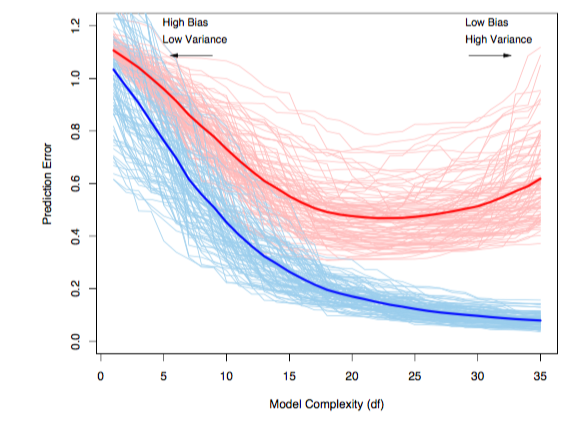
\includegraphics[width=0.7\columnwidth]{figures/figure-biasVariance/figure-biasVariance}
\caption{\label{figure-biasVariance} Figure borrowed from \protect\textcite{hastie-elemstatslearn} P. 220. Curves are measures of the estimated prediction error for the different degrees of freedom in the model (number of features). Blue curves correspond to the training error and red curves are for the test error. The bold curves are calculated by averaging over all of the colored curves.%
}
\end{center}
\end{figure}

In \ref{figure-biasVariance}, the authors fit a regression model on data to illustrate the interaction between bias and variance. The model increases complexity when using a greater number of features as more parameters need to be fit during the optimization procedure. Thus the model increases in complexity, as measured in its degrees of freedom.

At first the bias of the model is high both for the training and testing sets, and as a result we would expect to have a high generalization error. Then the overall error decreases as complexity increases. This behavior is expected because the model learns to better fit the data to give a better model output. We have that the expected prediction error, estimated by averaging over the test set' prediction error's, also decreases when the model's complexity is increased. However when the model starts to overfit the data, the test error starts to rise whilst the train error keeps decreasing. This situation is significant to our prediction error estimation cause it hinders that the model has lost predictive power due to an increase in variance.

In this situation, a common heuristic to select the best model is to stop increasing the model's complexity once the $EPE$ stops decreasing.

\subsection{ Using the Vapnik--Chervonenkis (VC) Dimension for prediction error estimation} \label{section-VcDimension}

%\textcite{vapnik-nature2013}
%\textcite{cherkassky-learning2007}

The Vapnik--Chervonenkis (VC) Dimension is a number based on a theoretical framework now called \textit{Statistical Learning Theory} (SLT). SLT is used to estimate the true expected prediction error from finite samples. Surprisingly, very few assumptions are needed and results are distribution independent. In addition, exact bounds are given for some common use cases with constructive analytical methods. For other cases authors propose sampling or experimental methods to estimate the VC dimension. For this part, most of the results and reasoning follows the works in \textcite{cherkassky-learning2007}. For a more broad development of this work, \textcite{vapnik-nature2013} is recommended too. Here we present a brief comment on the consistency of the training error to the prediction error and give example bounds for classification learners. In a supervised learning context, we use the empirical training ($\overline{err}$) or test errors ($\overline{err}_{test}$) to estimate the $EPE$.

Let $\mathrm{T} = (\textbf{X},\textbf{Y})$ be a training set of $n$ samples, $Y = \{0,1 \}$ and let $\mathcal {F} = \{f(x,\theta) \mid x \in X, \theta \in \Theta\}$ be a class of classifiers where $f_\theta: X \rightarrow Y \, \forall f \in \mathcal {F}$. This is a class of functions with domain over the input dataset $X$ and which are indexed by a parameter $theta$. This parameter will represent the index over the functions in $F$ and it will vary over all possible models attainable by our algorithm.

As an example, in logistic regression, $theta$ can be indexer by the values of each feature's weights $x^p$. The class $F$ will then represent the set of all possible functions from which to select the final model.
%In applications, a learner is fit from a class of functions.

As it was seen before in \ref{section-biasVariance}, a common problem in supervised learning when a particular learner is fit and then used to predict new values is overfitting. In practice this is common when $n$ is \textit{small} or when the number of features is \textit{large}.

In Vapnik and Chervonenkis's work, the focus is in the estimation of the prediction error through the convergence and consistency of the training error. They derive the VC dimension as an important value in determining convergence speeds for different machine learning algorithms. In this way, the SLT theory provides a theoretical framework to effectively characterize these dimensions in a constructive way. By the derived analytical bounds for a number of algorithms, we are enabled to estimate the distance between the empirical error and the generalization error.

Incorporating the loss functions directly in the model, SLT looks at functions of the form $Q(t,\theta) \ = \ L(f_\theta(x,y))$. Seen as a two variable function where $t=(x,y)$ represents the input and output data, and $theta$ the class index.

SLT theory focuses on functions which seek to minimize a certain functional characterized by the form of the loss function. Here, the $EPE(\theta)$ for any model takes the functional form

\begin{equation}\label{vapnik-risk}
\begin{split}
EPE(\theta) = & \ \Expect_{\textbf{t}} \left[  Q(t,\theta) \right]\\
= & \int Q(t,\theta) p(t) dt  \\
= & \int L(f_\theta(x),y) p(x,y) dx dy
\end{split}
\end{equation}\footnote{For simplicity, we will assume the functions $Q$ in the class to be bounded.}

where we let $p(t)$ be the \textbf{true} underlying probabilty function of the data.

However, as it was said before, we only have access to restricted data and we would like to estimate the risk functional for that class with the available training/test error. In this framework, this is what is called the empirical risk:

\begin{equation}\label{vapnik-empiricalRisk}
Err_{train}(\theta) =  \sum_{i=1}^n Q(t_i,\theta)
\end{equation}

Note that the learner is estimated directly from the risk functional. The loss function is put together with the approximating function and takes a strong part in the minimization procedure. On the other hand the unknown true underlying distribution $p(t)$ will not be estimated to minimize the functional and all of the effort will be put in directly using the training error as \textit{good} substitute for the prediction error.


We know that  training error depends on the model learned from the data and in turn, this depends on the sample. Due to this non-deterministic aspect of the problem, we will have different output  models for varying input samples, and even sometimes for the same sample. However, as we increase the sample size, we would still want to have the training error converge and to be consistent with the prediction error of the models.

%and $\theta^{*}_n$


\begin{definition}{Consistency of the Training error}

Let $\{\mathcal {T}_1, \mathcal {T}_2, ..., \mathcal {T}_n, ...  \}$ be a set of training samples such that $\forall n \ |T_n|=n$. Given a training sample of size $n$ and a class of learners $\Theta$, let $\theta^{*}_n$ be the argument minimizing the training error and let $\theta_0$ be the minimizing argument for the prediction error over the class of functions i.e. over all of the models of the class.

Then, the training error is said to be consistent if

$$\lim_{n\to\infty} Err_{train}(\theta^{*}_n) \  = \lim_{n\to\infty} EPE(\theta^{*}_n) \ =  EPE(\theta_0)$$

\end{definition}

The property of asymptotic convergence in the training and prediction errors is expected in any learning algorithm. In SLT, the consistency requires that the training and prediction errors'  sequences not only converge to the same values but that the sequence of minimal training errors also converge, to the minimizing value of the prediction error. At the same time, the sequence of prediction errors must converge to this same point.

In reality, it is natural to think that the approximation of the prediction error with the training error introduces a strong overestimation. The training error will also be biased by the sample used whilst the prediction error is given for the whole class and does not depend on the sample. Thus, in SLT theory, the minimization of the training error when using bounded loss functions is consistent if and only if:

%\begin{definition}{Uniform Consistency of the Training Error}

%\end{definition}
$$\forall \epsilon > 0 \ , \ \lim_{n\to\infty} P\left[ \sup_{\theta \in \Theta} \mid Err^{n}_{train}(\theta)  - EPE(\theta) \mid \right]  = 0 $$  % %     $$

% $$

Here the training error $Err^{n}_{train}(\theta)$ is the value of this error when using a sample of size $n$. In this sense, the training error is said to be consistent if it converges uniformly in probability over the whole class of functions\footnote{Remember that approximating functions in the SLT setting are indexed by the $\theta$ parameter.}. This implies that it characterizing the set of functions $Q(t,\theta)$ used to approximate the data will be important in finding an appropriate model. %SLT theory then introduces

The next results will be focused on a binary supervised machine learning setting. However the extension to other forms of supervised learning can be found in \textcite{cherkassky-learning2007}.

\begin{definition}{Shattering}

Let $\mathcal {A}= \{A_1,A_{2},\dots \}$ be a set family and $T$ a finite set. Let $t \subseteq T$, it is said that $\mathcal {A}$ picks out $t$ if there exists $A' \subseteq \mathcal {A} $ such that $ T \cap A' = t$. $T$ is said to be shattered by $\mathcal {A}$ if it picks out all of its subsets.

%The VC dimension of $\mathcal {A}$ is the biggest cardinality of a set shattered by $\mathcal {A}$.

\end{definition}

The n-th shattering coefficient $\Delta_n$ of a class $\mathcal {A}$ is defined to be the maximum number of subsets of $n$ elements picked out by the class.

If we consider a function from our set of classifiers, given a training set of size $n$
$\mathcal {T} = \{ t_1,t_2,...,t_n  \}$, we know that each classifier acts as an indicator function on the inputs $\{ x_1,x_2,...,x_n  \}$. The \textit{diversity} of this set of classifiers intuitively represents all of the different ways in which the input sample is partitioned by the classifiers.

We would say that $t$ is picked out by $\Theta$ if there exists a classifier $f_{\theta} \in \Theta$ such that $T = f_{\theta}^{-1}(\{1\})$. The classifiers in $\Theta$ define a unique mapping to the class of sets where each classifier is positive. It is said that $\mathcal {F}$ shatters a set $A$ if all of its subsets are picked out by the class of functions.

We will now reproduce the main necessary and sufficient conditions to have uniform consistency in predictive error approximation by our defined class of loss functions. Also,
Vapnik et al. provide bounds for the exponential convergence of this error. These bounds are constructive and can be effectively calculated in a number of commonly used models such as linear regressors and support vector machines. In addition, these bounds depend \textbf{only} of the structure of the approximators rather than the true distribution of the data.


\begin{definition}{Vapnik--Chervonenkis (VC) Dimension}

The Vapnik--Chervonenkis Dimension (VC) of a class of binary functions is the cardinality of the largest set which is shattered by $\mathcal {F}$. Note that by definition this means \textit{any} possible set shattered by $\mathcal {A}$.
\end{definition}\footnote{The VC dimension is briefly introduced here for the purpose of giving a theoretical approach to error estimation in machine learning methods. For a complete explanation on this topic refer to \textcite{vapnik-nature2013}}

The VC dimension gives a certain criteria for measuring the complexity of a class of binary functions by evaluating its expressiveness. The value, however, need not be finite.

As a simple example, one could use a linear regression of $d$ features $$g_{\theta} = \sum_{i=1}^d x_i \theta_i + \theta_0$$ as a classifier if we consider the indicator function of the positive half-plane induced by the regresssion: $$f_{\theta} = I(\sum_{i=1}^d x_i \theta_i + \theta_0 > 0)$$

This class of approximating functions can shatter up to $d+1$ samples, but no bigger sample. Thus the VC dimension is exactly $d+1$.

For more examples, refer to \textcite{cherkassky-learning2007} Pg. 113 for examples of different VC classes, finite and infinite.

SLT then proves that if a class of binary classifiers is of finite VC dimension, accurate bounds can be given to estimate train and predictive errors. For a sample of size $n$, take $Err^n_{train}(\theta^*)$ to be the minimum training error and $EPE(\theta_0)$ the minimum true predictive error.

They show that for classes which have a finite VC dimension $h$, the n-th shattering coefficient is bounded by a polynomial of order equal to the dimension
i.e. $\Delta_n(\mathcal {F}) \leq O(n^{h})$ \footnote{$O(\cdot)$ corresponds to Big-O notation.} where $VC$ stands for the VC dimension of the class.

Also, with probability at least $1 - \eta$ and $\forall \theta \in \Theta$

\begin{equation}\label{vapnik-classificationBound}
EPE(\theta) \leq  Err^n_{train}(\theta) + \frac{\epsilon}{2} \left(1 + \sqrt{1 + \frac{4 Err^n_{train}(\theta)  }{\epsilon}}  \right)
\end{equation}

where we have that $h$ is the VC dimension of the class and, when the approximating class $F$ is infinite of size $N$:
\begin{equation}\label{vapnik-epsilonBound}
\epsilon = a_1 \frac{h \left( ln(\frac{a_2 n}{h} ) -  ln(\frac{\eta}{4} ) \right)}{n}
\end{equation}

or

\begin{equation}\label{vapnik-epsilonBound}
\epsilon = 2 \frac{ ln(d) - ln(\eta)}{n}
\end{equation}

when $F$ is finite and consists of $d$ elements.

In the previous equations, the values of constants $a_1$ and $a_2$ are related to the nature of the density function $p(t)$ of the data. However, its values are proven to be uniformly bounded for all distributions, with $a_1 \in (0,4 ]$ and $a2 \in (0,2 ]$.

As a last result, the authors show that a more precise bound can be given for the function that minimizes the empirical risk $Err^n_{train}(\theta^*)$. They show that with probability $1 - 2\eta$

\begin{equation}\label{vapnik-classificationBoundPrecise}
Err^n_{train}(\theta^*) - EPE(\theta_0) \leq  \sqrt{\frac{-ln(\eta)}{2n} } + \frac{\epsilon}{2}\left( \sqrt{1 + \frac{4}{\epsilon} } \right)
\end{equation}

These results prove that effective approximations of the prediction error can be given for most algorithms of finite VC dimensions. They also give a clear characterization of how model complexity is related to the prediction error estimation.

In practical applications though, use of estimates might be limited to the determination of the VC value, specially with algorithms which are more complex and expressive such as neural networks. Due to this limitation, we show in the next section a practiced approach which is an easier and direct heuristic used to estimate the $PE$.


\subsection{Cross Validation}:
 There are a number of approximating functions or algorithms to be used in classification problems and each of these have different configurations or setups that, when fitted, produce different learners. The differences among the configurations are controlled by the \textit{parameters} of the algorithm. The nature of each parameter might stem from computation or statistical variants in the algorithm used. One common example of this is the $\lambda$ penalization parameter in logistic regressions, where $\lambda$ controls the amount of weight to be put in the regularization term of the minimized function.

The objective of Cross Validation is to systematically explore the different configurations of tuning parameters and decide which learner is better for the task at hand. By comparing the estimated generalization error of each model, where models vary accordingly with the values of the tuning parameters, a value is given and then used to select the \textit{best} model in the class.

This technique is one of the most widespread to evaluate the generalization performance of a set of learners. Given a number of possible configurations or values for the tuning (hyper) parameters of an algorithm, we would like to decide which selection of these fit the best estimator, as measured by the generalization error. In most cases data is generally scarce. At the same time prediction error estimates are based on asymptotic or analytical results which hardly computable in pratice. Thus CV intends to prevent over-fitting by iteratively holding out a random part of the dataset and by measuring the predictive accuracy of the learner fit on data \textit{in-sample} against new values from the \textit{hold-out} part of the dataset. The accuracy measure here is weighted by the loss function, which must be selected beforehand.

In this procedure, a partition of the samples is called a \textit{fold}. CV then partitions data into $K$ random folds, where the number $K$ has to be previously decided.\footnote{ We assume here that a random sample of the initial dataset was already left out in order to test the model's accuracy at the end. We refer to this set as the \textit{testing set}.} Let $\gamma : \{1,..,N\} \mapsto \{1, .., K\}$ be a function mapping samples to folds. Without loss of generality,  let $\alpha$ be an index of the model's hyper-parameters, where each distinct combination of the tuning parameters is identified by this index. Note that the domain of $\alpha$ will vary with the type of approximating function o algorithm used to learn.

 The CV algorithm now runs iterations over all of the folds, and takes one fold $\gamma^{-1}(\{k\})$ to be the validation set, where $k \in [1,...,K]$ is the indexer of the iteration. $\hat{f}^{-k}$ will denote the fitted estimator on the training set with the $k$-fold hold out and its classification performance will be tested against the \textit{out of sample} estimates. This means that for every sample in this $k$-fold, we measure the loss $L(y_i, \hat{f}^{-\gamma(i)}(x_i))$ of the model's prediction against the true target value.

Cross validation intends to estimate the expected \textit{out-of-sample} error $\Expect \left[  L(Y, \hat{f}(X)) \right]$, when the model is tested against \textbf{independent} samples from the true distribution. For this reason, it is fundamental to ensure independence of the training set and the test set. Any transformations that must be done on the input data that jointly uses the input and output samples in the process must be done and \textit{learned} only on the training set. This is because we mustn't introduce information from our test set in the estimator as the model should never \textit{see} the test data until we use it to evaluate our learner.

\textbf{Tuning-parameters (hyper-parameters) Selection}:

 Let $\mathcal{A} = [\alpha_0, \alpha_1,..., \alpha_l   ]$ be a list of hyperparameter settings and  $\mathcal{K} =[1,..,K]$ a list of folds.  A full K-Fold Cross Validation procedure takes the following form.

  \begin{algorithm}%[h]
  \SetAlgoLined
  \KwResult{Write here the result }
  Initialize $\mathcal{A}$ and $\gamma(\cdot)$\;
  \For{ $\alpha \in  \mathcal{A}$}{
  \eIf{data transformation}{
  Perform data transformation on the whole training set \;
  }{
  continue\;
  }
  \For{ $k \in  \mathcal{K}$}{
  fit $\hat{f}^{-k}(\cdot, \alpha)$\;
  }

  compute $CV(\alpha) = \frac{1}{N} \sum^n_{i=1} L\left( y_i, \hat{f}^{-\gamma(i)}(x_i, \alpha) \right)$\;
  }
  \caption{K-Fold Cross Validation Estimation Procedure}
 \end{algorithm}

Note that during the loop, each sample's prediction was tested on the model which was fitted without using that sample.

From the \textbf{CV} procedure it makes sense to choose a final  model $\hat{f}_\alpha$ with the lowest $CV(\alpha)$ value among all of possible hyperparameters. However, following ideas detailed in \ref{section-VcDimension}, importance is also given to the \textit{complexity} of the approximating function. A common rule of thumb is to favor models with a lower number of hyper parameters or number of features. In practice though, a class of approximating functions might have a defined complexity which is not analytically computable. Thus in some cases, crude heuristic estimates or common sense are used to estimate model complexity, without making use of theoretical arguments.

\subsubsection{Choice of $K$ parameter}

Experimental results show the differences among CV routines used with varying $K$ values. In synthetic and actual dataset , \textcite{hastie-elemstatslearn} P. 243, have found that using a \textit{higher} value for $K$, relative to the size of the dataset, means having a bigger training fold since each left-out partition is only $\frac{N}{K}$ in size. The results show models with good bias but high variance which is in accordance with the small size of the validation set. Note that having a higher value for $K$ will effect to a higher computational burden since $K$ estimators need to be fitted.

Having a lower $K$ value means using a smaller training set. Then it is common to find models with lower variance and higher bias. Empirical results also tend to show that the $EPE$ is overestimated. This is because having less available data to fit the model, implies having worse estimates from asymptotic results.

One last common choice for $K$ is $N-1$. This scenario is known as \textit{leave-one-out CV} and is a very used format in problems where data arrives sequentially over time. Here, samples of the training set $t_i = ( \boldsymbol{x_i} , \boldsymbol{y_i} )$ are accessible only in an order fashion. For these cases model evaluations are made against the new sample and the training set is updated with every arrival..\footnote{Note that here we must assume the \textit{exchangeability} of samples. This means that the distribution of the training set is not altered by a permutation of samples $F(x_1,...,x_n ) = F(x_\sigma{1},...,x_\sigma{n})$ for any random permutation $\sigma$ of the samples  }


A good survey and explanation of the drawbacks of the $K$-Fold CV estimator can be found in \textcite{bengio-unbiasedCvEstimator}. The authors prove that there is no distribution-free estimator unbiased estimator of the $K$-Fold cross validation estimator's variance. The theoretical arguments focus on the idea that error correlations between the training and validation sets are not taken into account by the CV procedure. These correlations are known and understood for the general case, but their estimation is not possible. As a consequence of this, comparison between different possible models is is hindered.

Empirical examples are built from synthetic datasets to show the shortcomings of the cross validation's algorithm which might show high deviations from its central value. Some exceptions appear though, specifically where distribution-free bounds can be found for a class of approximating functions. But these cases are specific only for this class. In general these bounds are not known, so using an unknown deviation of the CV estimator will affect the evaluation of different models.

Consensus \footnote{\textcite{hastie-elemstatslearn} P. 260} is that in general CV is a good procedure to estimate the expected prediction error with the training set fixed, but not good for the prediction error, conditional on the training set $\mathcal{T}$ fixed.



\subsubsection{CV Scores in Classification Learning}

In binary classification, the contingency table summarizes all of the learner's training performance. This shows the count the amount of samples that fall into one of the four groups derived from the comparison between the model's output and the observed data for the labels.

 Let $\hat{f}$ be our fit model, from the data with a CV procedure. Every sample has a target value $y$ and a predicted outcome $\hat{y}$ and there are only four possible outcomes for these two variables with two values for each.  We can express the models' target outcomes $\hat{y}$ into the positive ($\hat{P}$) or negative ($\hat{N}$) categories and the same with actual target data into the positive ($P$) or negative ($N$) categories.

To assess the performance of the classification algorithm and chose the \textit{best} model we must decide on how the CV procedure will value two different models. The idea is to quantify the mismatch between the target  and the predicted value. Here loss functions are also known as \textit{scores}, \textit{measures} or \textit{utility functions} and are built by looking at how many times an algorithm  misclassifies instances and where is the misclassification happening. To visualize this, a \textit{confusion} table with the following format is drafted:

\noindent
\renewcommand\arraystretch{1.5}
\setlength\tabcolsep{0pt}
\begin{tabular}{c >{\bfseries}r @{\hspace{0.7em}}c @{\hspace{0.4em}}c @{\hspace{0.7em}}l}
\multirow{10}{*}{\parbox{1.1cm}{\bfseries\raggedleft Target\\ value $y$}} &
& \multicolumn{2}{c}{\bfseries Predictive value $\hat{y}$} & \\
& & \bfseries \^{P} \ $(0)$ & \bfseries  \^{N} \ $(1)$   \\
& P \ $(0)$ & \MyBox{True}{Positive (TP)} & \MyBox{False}{Negative (FN)} &  \\[2.4em]
& N \ $(1)$ & \MyBox{False}{Positive (FP)} & \MyBox{True}{Negative (TN)} & \\
%& total & P \ $(0)$ &  &
\end{tabular}

In the confusion table, cell values count the amount of instances that fall into each of the four possible outcomes and scores are constructed from these values. The focus will be in measuring $FP$ and $FN$ volumes.

% to measure the algorithm's performance.
% Notice that the only correct cells are the $TP$ and $TN$ categories, each correctly classifying positive and negative samples
Some of the most used metrics include the following:

\begin{itemize}
\item \textbf{True Positive Rate  (Recall):} $\frac{TP}{P} = \frac{TP}{TP + FN}$ \\ This rate measures the percentage of real positive values captured by the algorithm. A high recall of the algorithm indicates that a high number of the real positive labels were classified as positive.


\item \textbf{Positive Predictive Value  (Precision):} $\frac{TP}{\hat{P}} = \frac{TP}{TP + FP}$ \\ This rate measures the \textit{overconfidence} of the algorithm in its predictions, a high precision indicates the value of the predictions.

\item \textbf{True Negative Rate  (Specificity):}  $\frac{TN}{N} = \frac{TN}{TN + FP}$ \\ This rate measures the percentage of real negative values captured by the algorithm.

\item \textbf{False Positive Rate  (Fall-Out):} $FPR = 1 - SPC$ \\ This rate measures the percentage of false negative values misclassified by the algorithm.

\item \textbf{Accuracy:} $\frac{TP + TN}{P + N} = \frac{TP}{TP + FP}$ \\ This rate measures the \textit{overconfidence} of the algorithm in its predictions.

%\item $F1_\beta$ \textbf{Score:} $(1 + \beta^2) \frac{TP + TN}{P + N} $ \\ This is the harmonic mean of the recall and the precision. It's advantage is that it can capture both of the scores in equal weight. Its values range in the $\[0,1 \]$ domain and are ordered in the sense that perfect classifiers have a $F1$ score of 1.
%
\item \textbf{F1  Score:} $\frac{TP + TN}{P + N} = \frac{TP}{TP + FP} = 2 \frac{1}{  \frac{1}{recall} + \frac{1}{precision}  }$ \\ This is the harmonic mean of the recall and the precision. It's advantage is that it can capture both of the scores in equal weight. Its values range in the $[0,1 ]$ domain and are ordered in the sense that perfect classifiers have an $F1$ score of 1.

\end{itemize}


\subsubsection{ROC Curve}

Even more metrics can be derived from the confusion table. Different interactions of the metrics can capture different aspects of an algorithm's classification performance.

One last important metric used widely in classification is the  \textbf{Area under ROC curve (ROCAUC)}. This metric applies only to algorithms which output for each sample  the probability of belonging to the positive class.  These methods then use a threshold value to to classify samples into the respective target classes. If we consider different values for this threshold, we will see that the recall and the fall-out of the algorithm will vary along different values.

As expected, there is an inverse relationships between these two as the threshold is varied. The ROC curve is defined as the relationship between these two values for different thresholds. The result is a curve defined in $[0,1]\times[0,1]$, referred to as the \textit{ROC space}.

To find a balance between these two rates, the ROCAUC metric measures the integral of this curve in ROC space. The score  calculated is thus known as \textit{Area Under the ROC Curve}. This metric follows the same properties as the ones mentioned before, where the best classifiers have values nearer to $1$.

The following figure shows an example ROC curve for an instance problem. Notice the algorithm's poor prediction performance where the ROCAUC is barely over the 'Luck' line. This line represents the performance of a \textit{random} classifier which arbitrarily labels samples as being to each possible class. It is expected to see good learners have better ROCAUC scores than the \textit{random classifier}.

\begin{figure}[h!]
\begin{center}
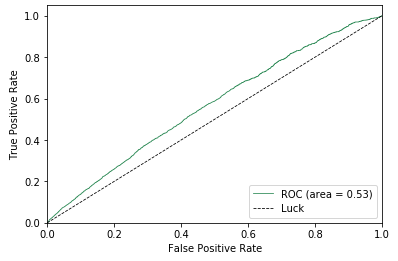
\includegraphics[width=0.7\columnwidth]{figures/figure-lowROCAUC/figure-lowROCAUC_original}
\caption{Example of a ROC curve from a Random Forest classifier used on the \textit{cancer} dataset.  The code used to build this graph is largely based on Python's Sci-kit Learn library. \protect\footnote{For more information on `sklearn` please refer to \url{http://scikit-learn.org/stable/index.html} \protect\textcite{sci-kit} . The cancer dataset is a copy of the UCI ML Breast Cancer Wisconsin (Diagnostic) set and is available from this same module or from \url{https://goo.gl/U2Uwz2}.}  }
\end{center}
\end{figure}
%

As a counter example, another algorithm was ran on the same problem as \ref{figure-lowROCAUC}.Notice how the algorithm is considered \textit{perfect} by the ROCAUC metric. No data transformation have been applied to the set between runs. The difference in the two scores is notable and corresponds entirely to the algorithm chosen.\footnote{The code used for this run can be found in a public iPython Notebook accessible at \url{https://github.com/jdemonasterio/authorea/blob/master/Notebooks/roc_curve_graph.ipynb}}

\begin{figure}[h!]
\begin{center}
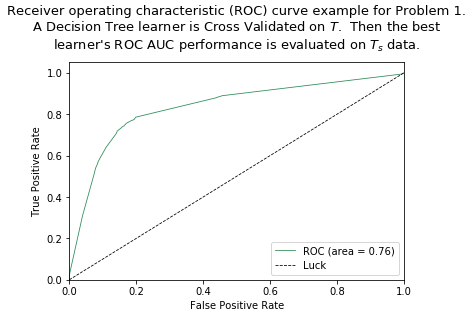
\includegraphics[width=0.7\columnwidth]{figures/figure-highROCAUC/figure-highROCAUC}
\caption{Example of a ROC curve from a Support Vector Machine classifier. The $0.97$ ROCAUC score given is now almost perfect for this problem.%
}
\end{center}
\end{figure}

\section{Classifier : Naive Bayes}

The Naive Bayes model encompasses a group of simple and computationally efficient algorithms which are based on a strong statistical independence among the features. Even though this assumption is in practice wrong, the model still achieves acceptable classification rates for some problems. In addition, it does not suffer in problems of high-dimensionality, where $p >> n$.

It is presented here mostly for computational benchmark purposes, where in practice the classification rate achieved by this model serves as a baseline for other, more complex, learners. Furthemore, the algorithm has linear  complexity in the number of features and samples $O(d+n)$, so it can be easlity extended to \textit{bigger} problem implementations. Furthermore, its maximum-likelihood estimation of the parameters has a closed form solution which is faster to compute over other iterative methods such as gradient descent techniques.

Let $x = (x_1,...,x_p)$ be any given data sample and $C_k$ be one of $K$ possible output classes of a classification problem. We take $p(C_k \mid x)$  to be the  class posterior probability of this class given the sample.

In section \ref{section-example}
we have used
\[
p(C_k| x) = \frac{P(x|C_k)P(C_k)}{P(x)}
\]\label{equation-posteriorProbabilties}

and argued that if our data is given, then our model can only improve the posterior probability by optimizing $P(x|C_k)P(C_k)$ which is just the joint probability of the sample and the class.

Here we can approximate the posterior as

\[
P(C_k \mid x) \approx p(C_k) * \prod_{j=1}^{p}    P(x_j \mid \bigcap_{k=j+1}^{p} x_k \cap C_k)
\]\label{equation-posteriorProbabilityDecomposition1}

We now impose a strong independence assumption among features, given the target class, to let the conditional probabilities factors become the probability of each feature. %This assumption is what gives the model its

This yields a posterior probability which depends only on the prior probability and on the individual likelihood of each feature.

\[
P(C_k \mid x) \approx p(C_k) * \prod_{j=1}^{p}    P(x_j | C_k)
\]\label{equation-posteriorProbabilityDecomposition2}

As we have said before, the parameters of the model can only reweigh the likelihood factors, so if we look to maximize the posterior probability, our final estimate of the posterior will take the following form.

\[
P(C_k \mid x) = \frac{1}{Z} p(C_k) * \prod_{j=1}^{p}    P(x_j | C_k)
\]\label{equation-posteriorProbabilityDecomposition3}

where in the equation $Z = p(x)$ is a scaling factor and is fixed to the dataset.

In practice, the model will stem into different algorithms where each variant will have a different probabilistic assumption on the likelihoods $p(x_j \mid C_k)$ of the model and on the priors $p(C_k)$. It is common to choose among using a nonparametric density estimations from the data or assuming that the data comes from an exponential family distribution such as a Gaussian, Bernoulli or Multinomial distributions. Different choices will certainly lead to different cross validation scores among problems. Altogether, these choices can be treated as part our model's hyperparamters and the best one can be selected with our CV procedure.
%Indeed,


Finally, the output class for a given sample will be given by taking the class $k'$ which maximizes the probability  $P(C_k' \mid x)$.

\section{Classifier : Decision Trees}

%rview of this supervised learner used in regression and classification problems.

% The models builds a
Decision trees are such as in the graph theoretical sense where each node acts as a rule to which any input sample can comply or not. The rules are built as linear (or similar) partitions of input space and they are built on the value of a given feature
%properties of the values for each feature.

At any6 given node the model takes a decision to include or exclude a sample $s$ from that partition by checking if $X_i(s) \in U$ where $X_i$ might be any given feature of the data and $U$ is a subset of said feature's space.

For numerical features, the input space $X$ willi be partitioned into  $L$ and $R$ where $L$ of the form $(-\infty,c]$.  The value $c \in \mathbb{R}$ is any given number predefined by the rule itself.   In the same way, for categorical features $L$ will be a subset of the possible values of that feature.

Altogether, a tree defines a partition of feature space in disjoint regions $A_1,...,A_K$ such that the tree's predicted output $\hat{y}$ for a sample $x$ is $c_k$ if the sample belongs to $A_k$. Here $c_k$ is one of the possible values taken by the target variable $y$ in the training set. And by the way trees were built, each $A_k$ is a hyper-rectangles in feature space.

In brief, the learner can be characterized by
\[
h(X) = \sum_{k=1}^K c_k I(X \in A_k)
\]\label{equation-decisionTreeModel}

where $c_k$ is the value that our model estimates for samples in the $A_k$ region. Both of these will have to be learnt by the model in the optimization procedure. %by minimizing its loss funciton.

By the points given above, the algorithm needs to determine what is the best way to split a set of samples that flow through a decision node. The \textit{goodness of split} will be measured by the loss metric of the algorithm. Here, the criteria used to decide on node splits are called \textit{node impurity measures}.
%them according, in order to optimize a loss metric.

%at each node
Most variations for this machine learning model build rules in a greedy fashion, where node impurity measures are locally optimized at each node to decide on which is the best splitting value. The reason for doing this is because not doing so will result in an algorithm whose computational complexity is infeasible. Given that the construction of optimal binary decision trees is NP-Complete \textcite{decisionTreesNP}, the optimal rules for the tree are then fit sequentially.

In conclusion, at any splitting node we have to find the \textit{best} feature $X^p$ and value split $t$ for which to partition the data in
$A_L = \{x \in \mathcal{T} \  / \ x^p \leq t \} $ and $A_R = \{x \in \mathcal{T}\  / \ x^p> t \} $. Let $N_l$ and $N_r$ be $|A_L|$ and $|A_R|$ respectively. Then, to quantify the \textit{best} feature for this split the algorithm minimizes:

%\frac{1}{N_{left}}
%\frac{1}{N_{right}}

\[
%\begin{split}
min_{p,t} \big[ min_{c_L }   \frac{1}{N_l}\sum_{x \in A_L(p,t) } L(y,c_L)        \ +   min_{c_R}   \frac{1}{N_r}\sum_{x \in A_R(p,t) }  L(y,c_R) \big]
%\end{split}
\]\label{equation-decisionTreeGreedyOptimization}

where $y$ is the target associated to our sample $x$ and $L(\cdot)$ is the loss function we have used to measure the quality of our split. Note that this can be done efficiently for a wide range of loss functions since the minimization can be done for each feature independently.

A tree is then grown in an iterative way from the top down \footnote{In this context the \textit{top} of a tree refers to the root of the tree.}, estimating the appropriate parameters at each rule split. All of the training set's samples would start at the top (the root node) and then travel down through the trees branches, in accordance to their fulfillment or not of each node's rule. A branch of the tree would stop growing once all samples at a node belong to the same target class.

Finally, we would have that the tree's leafs are the partition subsets over the input data and once a learner is fit, predicting targets for new samples is straightforward: the prediction of their target class will be the value given after traveling the sample down to its corresponding leaf node.

To illustrate this method, an instance is show in figure \ref{rf-treeFigure}. This classification tree example is built for the two class problem of gender prediction using data from CDRs:
%[.{\textit{Woman}}]
\smallskip
\begin{figure}[h]\label{rf-treeFigure}
\Tree[.{ $Calling\_Volume \leq 23$ } [.{$Province \in \{ San Luis, Chubut \} $} [.{$Time\_Weekend \geq 16$} [.{\textit{M}} ] [.{\textit{F}} ]  ]
[.{$Calls\_Weekdays \leq 48$}
[.{ $Time\_Weekday \geq 17$} [.{\textit{M}} ] [.{\textit{F}} ]] [.{\textit{F}} ] ]  ]
[.{$Calls\_Mondays \geq 2$} [.{$Province \in \{ Chubut, Cordoba \} $}  [.{\textit{M}} ] [.{\textit{F}} ] ]
[.{\textit{M}}  ]]]

\end{figure}

\smallskip

%[.{\textit{M}} ] [.{\textit{F}} ]

The most used metrics to build each rule are the \textit{Gini impurity measure} and the \textit{entropy} or \textit{information gain} criterion. The former optimizes for misclassification error in the two resulting sets. Where it values the accuracy of the model if all samples were to be tagged with the most common target-label in that split. The latter optimizes for information entropy, which is analogous to minimizing \textit{Kullback-Liebler divergence} of the resulting sets with respect to the original set previous to the split.

In decision trees, the process of iteratively partitioning the samples in splits continues until a predefined tuning parameter limit will stop the optimization or when there is only a single target class for all samples at the node.

The hyper-parameters for this model include the length of the tree,  the splitting rule threshold and the node impurity measures. From the descriptions previously given, we can list these directly:

\begin{itemize}
\item Max depth of the tree, or the number of allowed level of splits.
\item The criteria or measure used to select the best split feature at each node.
\item The leaf size or the total number of minimum samples allowed per leaf. Note that this is a limit imposed on  branch depth.
\item Number of features selected to decide on the best split feature at each node.
\end{itemize}


Intuitively, it is natural to find that trees of longer depth will overfit the data since more complex interactions among variables will be captured by refining the partition on input space. A trivial case would be to allow a tree to grow fully in depth and later assign to each sample in the training set its own region. This would yield a model with absolutely no bias but which will have a very high prediction error since new samples won't be labeled accordingly.

On the other hand having a tree which is too shallow will result in most cases in a biased algorithm.  This is because it results in an overly simple model incapable of correctly assigning labels.  We must then consider that the depth of a tree is a measure of the model's complexity and as such one of the most important hyperparameters of our model.

Another drawback of the model is the high variance instability. Authors point out that two very similar datasets can grow two very different resulting trees. This is due to the hierarchical nature of the splits, where errors randomly made in the first splits will be carried onward towards the leafs sinces samples continue down on a single branch.

The most common methods to control the tree's depth grow a very large tree $T_0$ that will continue until it reaches a depth limit threshold that is very unrestrictive. Then the tree will be pruned by removing branches and nodes to remove model complexity with only  a slight loss of accuracy.

To expand on this idea, let $T \subset T_0$ be a subtree of the first tree, where $T$ is obtained by pruning $T_0$.  Here the partition regions $R_j$ will be associated to $T$'s terminal nodes or leafs, indexed by $j$, which $j \in \{1,...,|T|  \}$.

Given a loss function, and a problem with $K$ possible target classes, we can define the following values:
\begin{equation}
\begin{split}
N_j & =  \mid\{x \in R_j \}\mid\\
\hat{p}_{jk} & = \frac{1}{N_j} \sum_{x \in R_j}  I(y=k)\\
c_j & =  argmax_{k} \  \hat{p}_{jk} \\
\end{split}
\end{equation}\label{decisionTreePruneParameters}

As we have mentioned before, at each split we use the node impurity measure to quantify this action. Here, we will denote $Q_j(T)$ to be the impurity measure for region $j$. In addition, we list the three most used impurity measures of classification trees:

\begin{itemize}
\item Misclassification error: $ \displaystyle \frac{1}{N_j} \sum_{x \in R_j}  I(y\neq c_j)  = 1 - c_j $
\item Gini index: $ \displaystyle \sum_{k\neq k'} \hat{p}_{jk} \hat{p}_{jk'}   = \sum_{k=1}^{K} \hat{p}_{jk} (1 - \hat{p}_{jk})  $
\item Cross-entropy: $ \displaystyle \sum_{k=1}^{K} -log(\hat{p}_{jk})\hat{p}_{jk} $
\end{itemize}


As an extension to the Gini index, it is also common to use a reweighted version of the sum. A loss matrix is multiplied to the factors in each summand. The matrix is reassigning weights to different cases of misclassification. Indeed, these weights become practical when we have that a sample from class $k$ incorrectly assigned to class $k'$ might be less important than other misclassifications.

Let $L \in \mathbb R_{\ge 0}^{K \times K}$ where $(L)_{(k,k')}$ is the cost of misclassifying a class $k$ sample into $k'$. Naturally we have that $L$ is a null diagonal matrix. Then the Gini index's summands will take the reweighted form  $L_{kk'} \hat{p}_{jk} \hat{p}_{jk'}$.

For the binary (two class) case $Q_j(T)$ can be expressed in simpler terms. If we consider $p$ to be the probability of success, then we have

\begin{itemize}
\item Misclassification binary error: $1 - max(p, 1-p)$
\item Gini binary index: $ 2p(1-p) $
\item Binary cross-entropy: $ -log(p)p - log(1- p)(1-p) $
\end{itemize}\label{decisionTreeCostFunctions}

In summary, we will have an impurity measure for each region $R_j$ and the altorithm will then aggregate all of them into a single measure called the \textit{cost complexity criterion}. The idea is that this loss function, as a function of a tree, will control the whole optimization procedure through the tree's parameters. The criterion will be managed to control the final model's bias and variance. We define it in the following way

\begin{equation}
C_\alpha(T)  = \sum_{j=1}^{|T|} N_j Q_j(T)  + \alpha|T|
\end{equation}\label{decisionTreeCostComplexity}


Here  $\alpha \in \mathbb{R}_{\geq 0}$ is a tuning parameter that values the trade-off between the tree complexity, as given by its depth, and the accuracy of the model as given by the measure we proposed in \ref{decisionTreeCostFunctions}. The idea is that given an $\alpha$ we find the subtree $T_{alpha} \subset T_0$ that minimizes \ref{decisionTreeCostComplexity}.

There are various methods we could use to find the optimal subtree. As an example, here we give an example of the \textit{weakest link pruning} algorithm which goes as follows:
%must \textit{prune} the initially grown tree

Let  $B(T)  = \sum_{j} N_j Q_j(T) $ be our pure loss function, without any complexity cost added. \textcite{breiman-cart84} shows that we can find $T_{alpha}$ included in a sequence of trees built for this. This sequence is constructed by iteratively pruning the node $j$ that, when removed from the tree, creates the smallest increase in $B(T)$.

In this way, we'll have a sequence of trees $T_0,T_1,...,T_l$ and a sequence of nodes $j_0, j_1,...,j_l$ respectively the ones minimizing the increase in $B(T_0),B(T_1),...,B(T_l)$ at each step. The algorithm will stop when have reached the root node and we will find our tree $T_{alpha}$ by comparing all of the $C_\alpha(T)$ for all of the trees built in the sequence. In practice, it is common to have this procedure done within a $K$-fold cross validation routine to reach to an estimated $\hat{\alpha}$.

For a more complete explanation of a decision tree for classification or regression problems, please refer to \textcite{breiman-cart84}.

\textit{}

\subsubsection{ Random Forests: Formulation }


Let $K$  be the number of trees in the ensemble and let $\Theta_k$ encode the parameters for the $k$-th tree. As we have mentioned before, there are various variants to the model and these variants will define the type encoding of the $\Theta_k$ parameters. In this part, we will not specify the type of forest used since the following proofs apply to all.

We denote $h(\textbf{x},\Theta_k)$ to be the corresponding classifier and $N$ the number of samples in the training set. The creation of a random forest involves an iterative procedure where at the $k$-th step, the parameter $\Theta_k$ is fit from the same distribution but independently of the previous parameters $\Theta_1, \ ..., \ \Theta_{k-1}$. %$\Theta$ will be encoded by a vector of randomly drawn integers from 1 to $M$ which is part of the model's hyperparameters.


Let $\{h_k(\textbf{x})\}_{i=1}^K$  \footnote{There is an abuse of notation by noting trees as $h_k(\textbf{x}$ and not $h(\textbf{x}, \Theta_k)$ } be a set of classifying trees and let $I$ denote the indicator function.  Define the margin function as

$$mg(\textbf{x},\textbf{y}) =  \frac{1}{K}   \sum_{k=1}^K I(h_k(\textbf{x}) = \textbf{y})
- max_{j\neq \textbf{y}}\left(\frac{1}{K} \sum_{k=1}^K I(h_k(\textbf{x}) = j) \right) $$ \label{eq:rf-marginFun}

%\end{equation}

The margin function measures, in average, how much do the trees vote for the correct class in comparison to all other classes. It is the training error of the model when using the misclassification loss. Here the generalization error is denoted as $PE*$ and is equal to  $$P_{\textbf{x}, \textbf{y} }(mg(\textbf{x},\textbf{y}) <0)$$

 It can be shown that, for $K$ sufficiently large, the generalization error under the misclassification loss converges to

$$ P_{\textbf{x}, \textbf{y} } ( P_{\Theta} (h(\textbf{x}, \Theta) = \textbf{y}) - max_{j \neq \textbf{y}} P_{\Theta} (h(\textbf{x}, \Theta) = j) < 0) $$

almost surely for all sequences of parameters $\Theta_1, ..., \Theta_k,...$

\subsubsection{Proof}
The proof follows from seeing that given a training set, a tree $\Theta$ and a class $j$ then
$$\forall \textbf{x}   \ P_\Theta(h(\theta,\textbf{x}) = j) \ = \
\lim_{L\to\infty} \frac{1}{L} \sum_{l=1}^K I(h_l(\textbf{x}) = j) \  $$
almost surely.

This is because if we look at the nature of the tree, we see that the set $\{\textbf{x} / h_l(\textbf{x}, \Theta) = j \}$ is built as a union of hyper-rectangles partitioning feature space. And given the finite size of the training set, there can be only a finite set of these unions of hyper-rectangles for all of the input data. Let $S_1, ..., S_M$ be an indexation of these unions and define $\phi(\Theta) = m $ if $\{\textbf{x} / h(\textbf{x}, \Theta) = j \} = S_m$.

We denote by $L_m$ the number of times that $\phi(\Theta_l) =m $, where $l \in {1...L}$ and $L$ is the total number of trees of this forest.

It is immediate that

\begin{equation}\label{rf-PEconvergence1}
\frac{1}{L} \sum_{l=1}^L I(h_l(\textbf{x},\Theta) = j) \ = \  \frac{1}{L} \sum_{m=1}^M L_m I(\textbf{x} \in S_m)
\end{equation}
%$$   $$

and that following the law of large numbers, there is a convergence almost everywhere of
\begin{equation} \label{rf-PEconvergence2}
\frac{L_m}{L} = \frac{1}{L} \sum_{l=1}^L  I(\phi(\Theta_l) = m)  \xrightarrow[L \to \infty]{}   P_{\Theta}(\phi(\Theta)= m).
\end{equation}
%$$ $$.

If we let $C = $ $\bigcup\limits_{m=1}^{M} C_{m}$ where each $C_m$ are zero-measured sets representing the points where the sequence is not converging.  If we combine \ref{rf-PEconvergence1} and \ref{rf-PEconvergence2}, we will finally have that  outside of $C$,

$$ \frac{1}{L} \sum_{l=1}^L I(h_l(\textbf{x}) = j) \xrightarrow[L \to \infty]{} \sum_m^M    P_{\Theta}(\phi(\Theta)= m) I(\textbf{x} =j ) \ = \ P_{\Theta}(h(\textbf{x}, \Theta) = j)  $$



\subsubsection{Predictive error bounds}

Random Forests are built upon a bag of weaker classifier, of which each individual estimator has a different prediction error. To build an estimate of the generalization error on the ensemble classifier, these individual scores and the irelationship between them must measured. In this sense, the \textit{strength} and \textit{correlation} of a Random Forest must be analyzed to arrive on an estimate of the generalization error.

%\begin{lemma}
%Given two line segments whose lengths are $a$ and $b$ respectively there is a
%real number $r$ such that $b=ra$.
%\end{lemma}

\begin{theorem}
There exists an upper bound for the generalization error.
\end{theorem}


\begin{proof}
Define $\hat{j}(\textbf{x},\textbf{y})$ as $arg max_{j\neq \textbf{y}} P_{\Theta}(h(\textbf{x}) = j)$ and let the margin function for a random forest (not a group of classifiers) be defined as

\begin{equation}\label{eq:rf-marginFunRf}
mr(\textbf{x},\textbf{y}) =  P_{\Theta}(h(\textbf{x}) = \textbf{y}) - P_{\Theta}(h(\textbf{x}) = \hat{j})
\\
= \Expect_{\Theta} \left[  I(h(\textbf{x},\Theta ) = y ) - I( h( \textbf{x},\Theta ) = \hat{j} )  \right]
\end{equation}


%\begin{equation}%\end{equation}

%\end{equation}

Here the margin function is described as the expectation taken over another function which is called the \textbf{raw margin function}\label{eq:rf-rawMarginFun}. Intuitively, the raw margin function takes each sample to be $1$ or $-1$ according to whether the ensemble classifier can correctly classify or not the sample's label, given $\Theta$.

With these definitions, it is straight to see that

%\begin{equation}%\end{equation}
$$mr( \textbf{x},\textbf{y} )^2 = \Expect_{\Theta, \Theta'} \left[ rmg( \Theta,\textbf{x},\textbf{y} ) \ rmg(\Theta',\textbf{x},\textbf{y} )  \right] $$.

This in turn implies that

\begin{equation}\label{eq:rf-marginFunVar}
\begin{split}
var(mr) & =  \Expect_{\Theta, \Theta'}
\left[
cov_{\textbf{x},\textbf{y}}
(rmg(\Theta,\textbf{x},\textbf{y} )rmg(\Theta',\textbf{x},\textbf{y} ))
\right] \\
& =  \Expect_{\Theta, \Theta'}
\left[
\rho(\Theta, \Theta')\sigma(\Theta)\sigma(\Theta')
\right]
\end{split}
\end{equation}

where $ \rho(\Theta, \Theta')$ is the correlation between $rmg(\Theta,\textbf{x},\textbf{y})$ and $rmg(\Theta',\textbf{x},\textbf{y})$, and $\sigma(\Theta)$ is the standard deviation of $rmg(\Theta,\textbf{x},\textbf{y})$. In both cases, $\Theta$ and $\Theta'$ are given.% to be fixed.

Equation \ref{eq:rf-marginFunVar} in turn implies that

\begin{equation}\label{eq:rf-varianceBound}
\begin{split}
var(mr) & =  \overline{\rho} (\Expect_{\Theta}\left[ \sigma(\Theta)\right] )^2 \\
& \leq  \overline{\rho} \Expect_{\Theta} \left[ var(\Theta) \right]
\end{split}
\end{equation}

where we have conveniently defined $\overline{\rho}$ as

\begin{equation}\label{eq:rf-meanCorrelation}
\frac{\Expect_{\Theta, \Theta'} \left[ \rho(\Theta, \Theta') \sigma(\Theta) \sigma(\Theta')\right]}
{\Expect_{\Theta, \Theta'} \left[ \sigma(\Theta) \sigma(\Theta')\right]}
\end{equation}

Note that this is the mean value of the correlation.

Let the strength of the set of weak classifiers in the forest be defined as

$$s =  \Expect_{\textbf{x},\textbf{y}} \left[ mr(\textbf{x},\textbf{y} ) \right] $$.\label{eq:rf-strength}

Assuming that $s \geq 0$ we have that the prediction error is bounded by
\begin{equation}\label{eq:rf-predictiveErrorBound1}
PE^* \leq var(mr)/s^2
\end{equation}
by Chebyshev's inequality. On the other we also have that


\begin{equation}\label{eq:rf-expectedVarBound}
\begin{split}
\Expect_{\Theta} \left[ var(\Theta) \right]  & \leq \Expect_{\Theta} \left[ \Expect_{\textbf{x},\textbf{y}}\left[ rmg(\Theta,\textbf{x},\textbf{y})   \right]  \right]^2 -s^2  \\
& \leq 1-s^2
\end{split}
\end{equation}


We can use  \ref{eq:rf-varianceBound}, \ref{eq:rf-predictiveErrorBound1} and \ref{eq:rf-expectedVarBound} to establish the upper bound for the prediction error we are looking for
\begin{equation}\label{eq:rf-PEBound}
PE^* \leq \overline{\rho}\frac{(1-s^2)}{s^2}
\end{equation}
\end{proof}

This bound on the generalization error shows the importance of the strength of each individual weak classifier in the forest and the correlation interdependence among them. The author of the algorithm \textcite{breiman-randomforests} remarks here that this bound may not be strong. He also puts special importance on the ratio between the correlation and the strength $\frac{\overline{\rho}}{s^2}$ where this should be as small as possible to build a strong classifier.
\subsubsection{Binary Class}
In the context of a binary class problem, where the target variable can only take two values, there are simplifications to the formula \ref{eq:rf-PEBound}. In this case, the margin function takes the form of $2 P_{\Theta}(h(\textbf{x}) = \textbf{y}) -1$ and similarly the raw margin function results in $2 I(h(\textbf{x}, \Theta) = \textbf{y}) -1$.


The bounds prediction error bounds derived in \ref{eq:rf-predictiveErrorBound1} assume that $s >0$ which in this case results in
$$ \Expect_{\textbf{x},\textbf{y}} \left[ P_{\Theta}(h(\textbf{x}) = \textbf{y}) \right] > \frac{1}{2} $$

Also, the correlation between $I(h(\textbf{x}, \Theta) = \textbf{y})$ and \  $I(h(\textbf{x}, \Theta') = \textbf{y})$, denoted $\overline{\rho}$ will take the form

$$ \overline{\rho} =  \Expect_{\Theta,\Theta'} \left[ \rho \left( h(\cdot{},\Theta) ,h(\cdot{},\Theta') \right)   \right] $$

\subsubsection{Other Notes on Random Forests}
One benefit of building Random Forest classifiers is that the algorithm easily increases the prediction error of a group of estimators by randomly building each of these in a way that decreases the variance of the overall model whilst trading a small loss in bias. The model is also robust to the introduction of a number of noisy features. If the ratio of informative to non-informative features is not extreme, selecting $m$ features at random at each split will mean that in most cases, splits will be made on those informative features. Note that in any given tree, the probability of drawing at least one informative feature in a split is still very high. This is because it follows a hypergeometric distribution $\mathcal{H}(P,j,l)$ with $l$ draws from a total population of $P$ features and only $j$ informative ones.

The depth of growth for each tree is another important tuning parameter. We must chose it correctly by assessing the model's performance across different values for $m$.  A deep tree will tend to overfit the data by partitioning input space to fit the training data. This effect will counter the overall reduction in variance of the forest and thus increase the generalization error of our algorithm.

%Therefore controlling the maximum allowed growth for the base learners will be important to improve the performance of the model.

The algorithm also benefits from a heuristic to measure variable importance.
A special modification in the way forests are built allows this to happen.

The idea for this is that at each split we can measure the gain of using a certain variable for the split versus not using it. Given a candidate feature $X_j$ to be analyzed and for every node in a tree where a split is to be done, we compare the improvement in the split performance, as measured by some pre-selected criteria, with and without $X_j$. These results are recorded and averaged across all trees and all of the split scenarios to have a score for the feature. The features with highest scores can be thought to be the most informative variables of the model.



\subsubsection{Random Forest Formulation}
Given $K$ number of trees, let $\Theta_k$ encode the parameters for the $k$-th tree and $h(\textbf{x},\Theta_k)$ the corresponding classifier. Let $N$ be the number of samples in the training set. The creation of a random forests involves an iterative procedure where at each $k$ step $\Theta_k$ is drawn from the same distribution but independently of the previous parameters $\Theta_1, \ ..., \ \Theta_{k-1}$ created at previous steps. $\Theta$ will be encoded by a vector of randomly drawn integers from 1 to $M$ which is part of the model's hyperparameters.


Let $\{h_k(\textbf{x})\}_{i=1}^K$  \footnote{There is an abuse of notation by noting trees as $h_k(\textbf{x}$ and not $h(\textbf{x}, \Theta_k)$ } be a set of classifying trees and let $I$ denote the indicator function.  Define the margin function as

$$mg(\textbf{x},\textbf{y}) =  \frac{1}{K}   \sum_{k=1}^K I(h_k(\textbf{x}) = \textbf{y})
- max_{j\neq \textbf{y}}\left(\frac{1}{K} \sum_{k=1}^K I(h_k(\textbf{x}) = j) \right) $$ \label{eq:rf-marginFun}

%\end{equation}
$ P_{\textbf{x}, \textbf{y} }(mg(\textbf{x}, \textbf{y}) < 0) $


The function measures, in average, how much do the trees vote for the correct class in comparison to all other classes and it can be shown that when $K$ is large then the prediction error converges almost surely to

$$ P_{\textbf{x}, \textbf{y} } ( P_{\Theta} (h(\textbf{x}, \Theta) = \textbf{x}) - max_{j \neq \textbf{y}} (\textbf{x}, \textbf{y}) < 0) $$

\subsubsection{Proof}
The proof follows from seeing that given a training set, a parameter $\Theta$ and a class $j$ then
$$\forall \textbf{x} \lim_{K\to\infty} \frac{1}{K} \sum_{k=1}^K I(h_k(\textbf{x}) = j) \ =   \ P_\Theta(h(\theta,\textbf{x}) = j) $$
almost surely.

By looking at the nature of each tree, $\{\textbf{x} / h_k(\textbf{x}, \Theta) = j \}$ denotes a union of hyper-rectangles partitioning feature space. And given the finite size of the training set, there can only be a finite set of these unions. Let $S_1, ..., S_K$ be an indexation of these unions and define $\phi(\Theta) = k $ if $\{\textbf{x} / h(\textbf{x}, \Theta) = j \} = S_k$.

We denote by $N_k$ the number of times that $\phi(\Theta_n) =k $, where $n \in {1...N}$ and $N$ is the total of trials.

It is immediate that

$$ \frac{1}{N} \sum_{n=1}^N I(h_n(\textbf{x}) = j) \ = \  \frac{1}{N} \sum_{k=1}^K N_k I(\textbf{x} \in S_k)  $$

and that there is a convergence almost everywhere of $$ \frac{N_k}{N} = \sum_{n=1}^N  I(\phi(\Theta_n) = k)  \xrightarrow[N \to \infty]{}   P_{\Theta}(\phi(\Theta)= k)$$.

If we let $C = $ $\bigcup\limits_{k=1}^{K} C_{k}$ where each $C_k$ are zero-measured sets representing the points where the sequence is not converging. We will finally have that  outside of $C$,

$$ \frac{1}{N} \sum_{n=1}^N I(h_n(\textbf{x}) = j) \xrightarrow[N \to \infty]{} \sum_k^K    P_{\Theta}(\phi(\Theta)= k) I(\textbf{x} =j ) \ = \ P_{\Theta}(h(\textbf{x}, \Theta) = j)  $$



\subsubsection{Predictive error bounds}

Random Forests are built upon a bag of weaker classifier, of which each individual estimator has a different prediction error. To build an estimate on the generalization error of the ensemble classifier, these individual scores and the inter-relationship between them must be taken into account. For this purpose, the \textit{strength} and \textit{correlation} of a Random Forest must be analyzed to arrive on an estimate of the generalization error.

%\begin{lemma}
%Given two line segments whose lengths are $a$ and $b$ respectively there is a
%real number $r$ such that $b=ra$.
%\end{lemma}

\begin{theorem}
There is an upper bound for the generalization error.
\end{theorem}

Define $\hat{j}(\textbf{x},\textbf{y})$ as $arg max_{j\neq \textbf{y}} P_{\Theta}(h(\textbf{x}) = j)$ and let the margin function for a random forest be defined as

\begin{equation}\label{eq:rf-marginFunRf}
mr(\textbf{x},\textbf{y}) =  P_{\Theta}(h(\textbf{x}) = \textbf{y}) - P_{\Theta}(h(\textbf{x}) = \hat{j})
\\
= \Expect_{\Theta} \left[  I(h(\textbf{x},\Theta ) = y ) - I( h( \textbf{x},\Theta ) = \hat{j} )  \right]
\end{equation}


%\begin{equation}%\end{equation}

%\end{equation}

Here the margin function is described as the expectation taken over another function which is called the \textbf{raw margin function}\label{eq:rf-rawMarginFun}. Intuitively, the raw margin function takes each sample to be $1$ or $-1$ according to whether the classifier can correctly classify or not the sample's label, given $\Theta$.

With these definitions, it is straight to see that

%\begin{equation}%\end{equation}
$$mr( \textbf{x},\textbf{y} )^2 = \Expect_{\Theta, \Theta'} \left[ rmg( \Theta,\textbf{x},\textbf{y} ) \ rmg(\Theta',\textbf{x},\textbf{y} )  \right] $$.

This in turn implies that

\begin{equation}\label{eq:rf-marginFunVar}
\begin{split}
var(mr) & =  \Expect_{\Theta, \Theta'}
\left[
cov_{\textbf{x},\textbf{y}}
(rmg(\Theta,\textbf{x},\textbf{y} )rmg(\Theta',\textbf{x},\textbf{y} ))
\right] \\
& =  \Expect_{\Theta, \Theta'}
\left[
\rho(\Theta, \Theta')\sigma(\Theta)\sigma(\Theta')
\right]
\end{split}
\end{equation}

where $ \rho(\Theta, \Theta')$ is the correlation between $rmg(\Theta,\textbf{x},\textbf{y})$ and $rmg(\Theta',\textbf{x},\textbf{y})$, and $\sigma(\Theta)$ is the standard deviation of $rmg(\Theta,\textbf{x},\textbf{y})$. In both cases, $\Theta$ and $\Theta'$ are given to be fixed.

Equation \ref{eq:rf-marginFunVar} in turn implies that

\begin{equation}\label{eq:rf-varianceBound}
\begin{split}
var(mr) & =  \overline{\rho} (\Expect_{\Theta}\left[ \sigma(\Theta)\right] )^2 \\
& \leq  \overline{\rho} \Expect_{\Theta} \left[ var(\Theta) \right]
\end{split}
\end{equation}

where we have conveniently defined $\overline{\rho}$ as

\begin{equation}\label{eq:rf-meanCorrelation}
\frac{\Expect_{\Theta, \Theta'} \left[ \rho(\Theta, \Theta') \sigma(\Theta) \sigma(\Theta')\right]}
{\Expect_{\Theta, \Theta'} \left[ \sigma(\Theta) \sigma(\Theta')\right]}
\end{equation}

Note this is the mean value of the correlation.

Let the strength of the set of weak classifiers in the forest be defined as

$$s =  \Expect_{\textbf{x},\textbf{y}} \left[ mr(\textbf{x},\textbf{y} ) \right] $$.\label{eq:rf-strength}

Assuming that $s \geq 0$ we have that the prediction error is bounded by
\begin{equation}\label{eq:rf-predictiveErrorBound1}
PE^* \leq var(mr)/s^2
\end{equation}
by Chebyshev's inequality. On the other hand it can also be noted that


\begin{equation}\label{eq:rf-expectedVarBound}
\begin{split}
\Expect_{\Theta} \left[ var(\Theta) \right]  & \leq \Expect_{\Theta} \left[ \Expect_{\textbf{x},\textbf{y}}\left[ rmg(\Theta,\textbf{x},\textbf{y})   \right]  \right]^2 -s^2  \\
& \leq 1-s^2
\end{split}
\end{equation}

\begin{proof}
We can use  \ref{eq:rf-varianceBound}, \ref{eq:rf-predictiveErrorBound1} and \ref{eq:rf-expectedVarBound} to establish the upper bound for the prediction error we are looking for
\begin{equation}\label{eq:rf-PEBound}
PE^* \leq \overline{\rho}\frac{(1-s^2)}{s^2}
\end{equation}
\end{proof}

This bound on the generalization error shows the importance of the strength of each individual weak classifier in the forest and the correlation interdependence among them. The author \textcite{breiman-randomforests} of the algorithm remarks here that this bound may not be strong. He also puts special importance on the ratio between the correlation and the strength $\frac{\overline{\rho}}{s^2}$ where this should be as small as possible to build a strong classifier.
\subsubsection{Binary Class}
In the context of a binary class problem, where the target variable can only take two values, there are simplifications to the formula \ref{eq:rf-PEBound}. In this case, the margin function takes the form of $2 P_{\Theta}(h(\textbf{x}) = \textbf{y}) -1$ and similarly the raw margin function results in $2 I(h(\textbf{x}, \Theta) = \textbf{y}) -1$.


The bounds prediction error bounds derived in \ref{eq:rf-predictiveErrorBound1} assume that $s >0$ which in this case results in
$$ \Expect_{\textbf{x},\textbf{y}} \left[ P_{\Theta}(h(\textbf{x}) = \textbf{y}) \right] > \frac{1}{2} $$

Also, the correlation between $I(h(\textbf{x}, \Theta) = \textbf{y})$ and \  $I(h(\textbf{x}, \Theta') = \textbf{y})$, denoted $\overline{\rho}$ will take the form

$$ \overline{\rho} =  \Expect_{\Theta,\Theta'} \left[ \rho \left( h(\cdot{},\Theta) ,h(\cdot{},\Theta') \right)   \right] $$

\subsubsection{Other Notes on Random Forests}
One benefit of building Random Forest classifiers is that the algorithm easily increases the prediction error of a group of estimators by randomly building each of these in a way that decreases the variance of the overall model whilst trading a small loss in bias. The model is also robust to the introduction of number of noisy features. If the ratio of informative to non-informative features is not extreme, selecting $m$ features at each split at random will mean that in most cases, splits will be made on those informative features. Note that in any given tree, the probability of drawing at least one informative feature in a split is still very high. This is because it follows a hypergeometric distribution $\mathcal{H}(P,j,l)$ with $l$ draws from a total population of $P$ features and only $j$ informative ones.

The depth of growth for each tree is another important tuning parameter. We must chose it correctly by assessing the model's performance across different values for $m$.  A deep tree will tend to overfit the data by partitioning input space to fit the training data. This effect will counter the overall reduction in variance of the forest and thus increase the generalization error of our algorithm.

%Therefore controlling the maximum allowed growth for the base learners will be important to improve the performance of the model.

A special modification in the way Random Forests are built, allows to derive a measure of variable importance. The idea for this, is that at each split we can measure the gain of using a certain variable for the split versus not using it. Given a candidate feature $X_j$ to be analyzed and fore every node in a tree where a split is to be done, we compare the the improvement in the split performance, as measured by some pre-selected criteria, with and without $X_j$. These results are recorded and averaged across all trees and all of the split scenarios to have a score for the feature. The features with the highest scores can be thought as the most informative variables of the model.



\section{Boosting Models}\label{section-boosting}
\subsection{AdaBoost}
\textcite{schapire-adaBoost}

Boosting methods are similar to additive methods such as in Random Forests because they combine the predictions of weak lerners to output the combined model's prediction. The full model is grown sequentially from base estimators such as decision trees, but the difference is that each new iteration tries to reduce the overall bias of the combined estimator. This provides greater predictive power when the base model's accuracy is weak. However, care must be taken to control the increase in variance.

In the AdaBoost variation of ensembling, each iteration builds a new weak learner which is set to improve on the samples misclassified by the weak learner before, rather than building a new uncorrelated learner. Weights are used to rank the samples by importance, where a sample with higher misclassification rate will receive a stronger weight. The name of the algorithm is derived from the term \textit{adaptive boosting}, where sample weights are updated at each iteration.

Tuning parameters in this algorithm are the same as those in the base learners. In addition, the number of steps that the algorithm will \textit{boost} is a new hyperparameter.

The chained construction of weak learners has its implications in computational complexity. Base learners are not constructed independently and as such, the parallelization of this algorithm is rarely possible. At the same time, the sequential optimization of learners improving on the one before marks a \textit{greedy} minimization approach of the general loss function.

These properties underline a substantial difference to Random Forests where base learners are built as uncorrelated as possible and where optimization can be performed globally, which allowed a significant parallelization of the algorithm.

\subsection{AdaBoost Formulation}

Let
\begin{equation} \label{equation-adaBoostTrainingError}
\overline{err} = \frac{1}{N} \sum_{i=1}^{N} I(y_i \neq \hat{y_i})
\end{equation}
%$$$$
denote the training set's misclassification error. As usual, $N$ is the amount of samples in our dataset, $y$ is our target variable and $\hat{y}$ is our model's prediction for the target, given the samples. We also take
$$\Expect_{X \ Y} [ I(Y \neq \hat{Y}(X)) ]$$

to be the expected error rate of the model on the true,  unknown distribution of the data.

Let $m$ index the iteration number in the AdaBoost algorithm. Set $w^{(m)}_i$ to be the $i$-th sample's weight. We will initialize this variable to be equiprobable at $w^{(0)}_i = \frac{1}{N} \forall i$. Let $h(x,\theta)$  denote our model's weak learner. With this notation, we assume the function to have domain in the input feature space and in the parameters defining the learner. Naturally these will depend on the problem structure and on the base learner. Then AdaBoost's model takes the following form:

\begin{equation} \label{equation-adaBoostModel}
\hat{y}(x) = \sum_{m=1}^{M} \gamma_m h(x,\theta_m)
\end{equation}

where $M$ is the model's hyperparameter indicating the amount of weak learners and thus the amount of iterations. Here, each $\theta_m$ will encode the base learner's parameters and $\gamma_m$ will denote the weight of that weak learner in the overall model.

The algorithm's iteration will build $\hat{y}$ starting from $\hat{y_i}^{(0)}= 0 \forall i$ and at each stage we will minimize a function that tries to correct the performance of the last model. At step $m$ we will search for $(\gamma_{m}, \theta_{m})$ where

\begin{equation} \label{equation-adaBoostIteration}
\begin{split}
(\gamma_{m}, \theta_{m}) = \underset{\gamma, \theta}{\mathrm{argmin}}  \sum_{i=1}^{N} & L\big( y_i,   \hat{y}^{m}(x_i) + \gamma h(x_i,\theta) \big) \\
= \underset{\gamma, \theta}{\mathrm{argmin}} \sum_{i=1}^{N}  & L\big( y_i,    \sum_{j=1}^{m} \gamma_j h(x_i,\theta_j) + \gamma h(x_i,\theta) \big)
\end{split}
\end{equation}

The greedy nature of the algorithm becomes explicit in the procedure above, where we have fixed all of the previous optimized values for $\gamma_j$ and $\theta_j$.

AdaBoost was first derived in \textcite{schapire-adaBoost} and it was introduced with a specific  minimizing function. The general version here presented allows the use of a broad range of base learners which need not to be from the same algorithmic family. In the first version introduced, the loss function used was the exponential loss which is $L(y,z) = e^{-yz}$ and the target variable took the values $1$ or $-1$.

This particular case yields a similar equation as in \ref{equation-adaBoostIteration}, but where

\begin{equation} \label{equation-adaBoostExponentialIteration}
\begin{split}
(\gamma_{m}, \theta_{m}) = \underset{\gamma, \theta}{\mathrm{argmin}}  \sum_{i=1}^{N} & exp\big( -y_i  (\hat{y}^{m}(x_i) + \gamma h(x_i,\theta) )\big) \\
= \underset{\gamma, \theta}{\mathrm{argmin}}  \sum_{i=1}^{N} & exp\big( -y_i  \hat{y}^{m}(x_i)\big) exp\big(- \gamma h(x_i,\theta)y_i \big)
\end{split}
\end{equation}


Given that we are only minimizing $\gamma$ and $\theta$, we can group $e^{-y_i  \hat{y}^{m}(x_i)}$ into a single value $w_i^{(m)}$ which we will set to the weight of each sample. This weight strongly depends on the past steps of the algorithm.  The equation now becomes

%We can also take the $\gamma$ factor out of the sum, since it is fixed for all samples.

\begin{equation} \label{equation-adaBoostExponentialIteration2}
(\gamma_{m}, \theta_{m}) = \underset{\gamma, \theta}{\mathrm{argmin}} \    \sum_{i=1}^{N}  w_i^{(m)} exp \big(-\gamma h(x_i,\theta)y_i \big)
\end{equation}

We can then minimize for $\theta$ first, independently of the value of $\gamma$. The series in \ref{equation-adaBoostExponentialIteration2} can be decomposed

\begin{equation} \label{equation-adaBoostThetaDecomposition}
\begin{split}
e^{-\gamma} \sum_{i \mid y_i = h(x_i,\theta)} w_i^{(m)}  + e^{\gamma} \sum_{i \mid y_i \neq h(x_i,\theta)} w_i^{(m)} & = \\
( e^{\gamma} - e^{-\gamma}) \sum_{i = 1}^{N} w_i^{(m)} I \big( y_i \neq h(x_i,\theta)   \big)  + e^{-\gamma} \sum_{i = 1}^{N}   w_i^{(m)} &
\end{split}
\end{equation}


and then the minimizing solution for $h(\cdot, \theta_{m+1})$ will be the one satisfying

\begin{equation} \label{equation-adaBoostThetaMinimization}
\theta_{m} = \underset{ \theta}{\mathrm{argmin}}  \sum_{i=1}^{N}  w_i^{(m)} I \big( y_i \neq h(x_i,\theta)   \big)
\end{equation}

Let $u = \sum_{i=1}^{N}  w_i^{(m)}$ and $v = \sum_{i=1}^{N}  w_i^{(m)} I \big( y_i \neq h(x_i,\theta)   \big) $, which are both constant in $\gamma$. Consider \ref{equation-adaBoostTrainingError} and note that $\frac{u}{v} = \frac{1}{\overline{err}}$. If we now solve for $\gamma$ in \ref{equation-adaBoostThetaDecomposition}, we can take

\begin{equation} \label{equation-adaBoostBetaMinimization}
f(\gamma) = ( e^{\gamma} - e^{-\gamma}) u +  e^{-\gamma}v
\end{equation}

which has a minimum at
\begin{equation}
\gamma_{m} = \frac{1}{2} log\big( \frac{1 - \overline{err} }{ \overline{err} }  \big)
\end{equation}

As seen by the equation above, the minimizing value for $\gamma$ is directly related to the training error of the algorithm for the \textit{whole} dataset. This weight will be reflected upon all samples in general and then we would expect this rate to decrease at every iteration.  Taking advantage of this closed form, the value is plugged into the next step of the AdaBoost procedure to update sample weights as

\begin{equation}
w_i^{(m+1)} =   w_i^{(m+1)} e^{\gamma_m(-y_i h_m(x_i))} \\
\end{equation}

In this way we have that the weights are updated for those samples which have a higher misclassification rate. This is a relevant aspect of the algorithm. At each step, more importance is given to misclassified samples over correctly classified ones.

%$-y_i h_m(x_i) = 2I \big( y_i = h_m(x_i)   \big) -1$ which means that $\gamma_m(-y_i h_m(x_i))$


The final form of the model is
$$  \hat{y}(x) = sgn\big(  \sum_{m=1}^{M} \gamma_m h_m(x) \big)$$ which outputs the most frequent prediction given by all of the weak learners. This is because all of the correct predictions will be greater than zero and negative values for the incorrect predictions. \footnote{This is when we consider the binary class case where $Y$ can take only $1$ or $-1$ values.}
%This particular property is what gives rise

At first the choice of the exponential loss function can seem arbitrary, but for the context of statistical learning this measure presents an important property where its minimizing function is the log-odds ratio of the two output classes:
$$f^*(X) = \underset{f}{\mathrm{argmin}} \  \Expect_{Y | f(X)}\big[ exp(-Yf(X))  \big] = \frac{1}{2}
log\big( \frac{ P(Y=1 \mid X) }{ P(Y=-1 \mid X) }  \big) $$


The use of the exponential loss function $exp(-Yf(X))$ is also desirable in this context since significantly more weight is put on misclassifications rather than on correct classifications. This is because the function is not symmetric in $Yf(X)$ and that having a correct classification will mean a factor of only $e^{-1}$, whilst on the other hand a misclassification will mean a factor of $e$.

A drawback of this loss though, is that it is not robust to outliers or to noisy data. During runtime weights are constantly shifting towards misclassified samples. Then if samples are mislabeled, this will make the algorithm repetitively focus on classifying incorrectly the data.



\subsection{Gradient Tree Boosting}

As explained before, the boosting method builds a high model learned from other \textit{weaker} learners. For the case of \textit{gradient tree boosting}, decision trees are used as base learners. If $Tr$ is a set of tree models and $K$ the number of trees in $Tr$, then trees will be the parameters for this model and at step $m$ the output will be

\[
\hat{y}^{((m)}=  \sum_t^m \gamma_t h_t(x) , \  h_t \in Tr \ \forall t \in {0...K}
\]

where $\gamma_t$ indexes the weight for each tree $h_t$ and $K$ is a hyper-parameter that represent the number of trees. Each new base learner is added to the model

\[
\hat{y}^{(m+1)} =   \hat{y}^{(m)}  + \gamma_m h_m(x)
\]

and the new base model is selected upon minimizing the misclassification rate of the full model at the previous step $m$, where a loss function previously selected is minimized to select the next best base learner:

\[
h_m(\cdot) = \underset{h,\gamma}{\mathrm{argmin}}   \sum_{i=1}^{n} L ( y_i,  \hat{y_i}^{(m-1)} -  \gamma h(x_i)  )
\]


For the moment, we include the tree's weight $\gamma$ as part of the weak learners in a single function $f_t(\cdot)$. Therefore the model results in,

\[
y =  \sum_k f_t(x) ,  \ f_t \in Tr  \ \forall t \in {0...K}
\]

where we represent a single tree with the form

\[
f(x) = \theta_{q(x)} = \sum_{j=1}^J \theta_j I(x \in  R_j)
\]

with $\theta_j \in \mathbb{R} \ \forall j = 1,...,J$ and $ \cup_{j=1}^J R_j$ a partition of feature space. The function $q : X \mapsto \{1,...,J\}$ denotes the mapping from samples to regions. In summary, $\{\theta_j, R_j\}_{j=1}^J$ are the weak model's parameters and $J$ is a hyper-parameter. Note that finding the best partition of feature space is a non-trivial optimization problem since finding subset partitions satisfying a global condition is a combinatorial feat.

For the high model, the objective function would account for the relationships among the trees and we would have that

\[ Obj(\Theta) = \sum_i^n l(y_i,\hat{y}_i))  +  \sum_t R(f_t) \] \label{eq:boositing-objfunction} \footnote{In the formula \ref{eq:boositing-objfunction} }
%

At this level $\Theta$ is a parameter encoding all of the base trees' model information. For each base tree $f_t$, $\theta_t$ is the parameter associated to it. This means that $\Theta =  \bigcup_{t \in {0...K}} \theta_t  \cup \theta_0$.  The parameter $\Theta_0$ is not associated to any tree but reserved to characterize the tree ensemble.

If an optimization routine were to collectively fit all of the parameters in $\Theta$ to learn this model, we would have a very computational complex model. In practice this would result in an prohibitive cost. Instead, we rely on optimization heuristics.

\subsubsection{Additive Training}

As usual, the first take on this optimization problem goes using a greedy optimization routine. One tree is fit at a time and new trees are then successively added in later steps to improve on previous trees' errors.

Let $t$ be the step indexer of the algorithm, where $t \in {0,..,K}$, $Obj_t(\Theta)$ be the objective function and $\hat{y}^t$ be the target variable respectively. Then the $i$-eth target's value at each step would iterate in the following way:

\begin{equation} \label{eq:gb-targetSteps}
\begin{split}
\hat{y}_i^0 = & 0 \\
... \\
\hat{y}_i^t = &\sum_{k=1}^{t} f_k(x_i) = \hat{y}^{t-1}_i +  f_t(x_i)
\end{split}
\end{equation}
%\sum_{i=0}^{\infty} a_i x_i
where each tree is added in such a way that we are minimizing

\begin{equation}
Obj^t(\theta) =  \sum_i^n L(y_i, \hat{y}^{t-1}_i +  f_t(x_i) ) + c(t) + R(f)
\end{equation}


Note that we have included here a regularization term (see section \ref{subsection-hyperParametersRegularization}) $R$ on all of the weak learners. For most cases,  this term will take the form of a Tikhonov regularization. This will add another complexity tuning parameter to control the length of the overall procedure $c(t)$ which is variable only in $t$.

If we assume we have sufficient conditions to approximate the objective function with second order Taylor approximation around $f_t(x_i)$,we would have

\begin{equation}\label{equation-gradientBoostingTaylor}
Obj^t(\theta) \approx \sum_i^n {L(y_i, \hat{y}^{t-1}_i) + g_i f_t(x_i,\theta_t) + \frac{1}{2} h_i f_t(x_i,\theta_t)^2 } +  R(f(\Theta)) +  c(t)
\end{equation}

Here $g_i$ and $h_i$ are first and second order approximations of the loss function with,

\[
g_i =  \frac{\partial L(y_i, \hat{y}^{t-1}_i)}{\partial \hat{y}^{t-1}_i}, \  \\
h_i =  \frac{\partial^2 L(y_i, \hat{y}^{t-1}_i)}{\partial (\hat{y}^{t-1}_i)^2 }
\]

Still, the equation \ref{equation-gradientBoostingTaylor} can be simplified by taking only the terms that are dependent on $\theta$. This also means replacing the actual tree's predictions for each sample as $\theta_{q(x_i)}$, where $q(\cdot): X \rightarrow leaf$ is the function that maps samples to the tree's leafs. Then,

%for that tree's evaluation.

\begin{equation} \label{eq:gb-objSteps1}
Obj^t(\theta) \approx  \sum_i^n {g_i \theta_{q(x_i)} + \frac{1}{2} h_i \theta_{q(x_i)}^2 } + \gamma ({t-1}) + \frac{1}{2}\lambda \sum_{j=1}^{t-1} \theta_j^2 \\
\end{equation}

As an example, we have already replaced the regularization terms $c(t)$ and $R(f)$ with penalties on the size of the ensemble and with an $l$2 penalty on the weight of each individual leaf.

If we rearrange the equation above we get

\begin{equation} \label{eq:gb-objSteps1}
\begin{split}
Obj^t(\theta) \approx  & \sum_{j=1}^{t-1} \left(  \sum_{i \in \{q(x_i)=j\}} (g_i )\theta_{j} + \frac{1}{2} \sum_{i \in \{q(x_i)=j\}} (h_i + \lambda ) \theta_{j}^2  \right) + \gamma ({t-1}) \\
\approx  & \sum_{j=1}^{t-1} \left(  \theta_{j}\sum_{i \in \{q(x_i)=j\}} (g_i ) + \frac{\theta_{j}^2}{2} \sum_{i \in \{q(x_i)=j\}} (h_i + \lambda )  \right) + \gamma ({t-1})
\end{split}
\end{equation}

which, as a function of $\theta$ is a quadratic equation if we assume $\gamma$ to be fixed. This results in a convenient and closed-from analytical formulation to select the the value at step $t$. In this sense, a direct greey optimization approach, such as gradient descent, can be used to find the tree $f_t(\theta)$ minimizing the previous expression.

As we have stated before the approach assumes that we have met enough smoothness conditions on the loss function with respect to the prediction variable
%$ \forall i \in {1...n}, \forall t \in {1..K}, \exists g_i(\hat{y}^{t}_i), h_i(\hat{y}^{t}_i) $
and that these values are effectively computable. This is why smooth loss functions play an important role here in providing a feasible method.

%\[
%Obj^t(\Theta) \approx \sum_i^n {  g_i f_t(x_i) + \frac{1}{2} h_i f_t(x_i)^2 } +  Obj_{t-1}(\Theta) + R(f_t) - R(f_{t-1})
%\]

%This equation form results in a direct method for a greedy optimization approach.  We will have to search for the tree $f_t$ that minimizes \\
%$\sum_i^n {  g_i f_t(x_i) + \frac{1}{2} h_i f_t(x_i)^2 } + R(f_t)$ at the $t$-th step.


As a last remark on boosting algorithms, there are two additional heuristics used to improve the generalization performance of boosting algorithms. The arguments in favor of these methods are rather experimental and not much theoretical, although their benefits are intuitive . The authors in \textcite{hastie-elemstatslearn} and \textcite{bishop-patternRecognition} mention them because of their overall contribution to the generalization error.

The first idea to reduce the overall variance of the algorithm is to subsample the data. This means that at each iteration, only a bootstrapped sample of the dataset will be selected to build the new weak learner. The motivation behind this is the same that as in Random Forest, where reducing the overall of available data to fit the new weak learner will most likely reduce the variance of the method. In practice, the rate of sampling will be controlled by a tuning parameter in the model.

The other heuristic is considered to be more important, at least experimentally by \textcite{hastie-elemstatslearn}. This is done by successively applying a \textit{shrinkage} factor $v \in  (0,1)$ to the new model.  At step $t$, instead of letting the overall model become $ \hat{y_i}^{(t)} = \hat{y_i}^{(t-1)} +  \theta_t h_t(x_i) $, we multiply the shrinkage factor $v$ to these values before adding them to the overall model at step $t-1$. This shrinkage factor is also known in the literature as the \textit{learning rate} of the algorithm.  Note that $v$  is reducing the movement of the algorithm in the direction of optimization provided by $\theta_t$ and $h_t$. In practice this results in longer iterations needed to reach the algorithm's \textit{best} prediction rate. However, when this factor is combined with subsampling, it has been empirically shown to improve the overall generalization accuracy.



asdf

$\Pi \Pi \Pi$


\section{Machine Learning in Practice: Technical Observations}\label{section-technicalObservations}
\textbf{TODO A desarrollar}
Python, sklearn, pandas, graphlab, etc

Data process raw data by reading in chunks from huge files (compressed filesizes amount to 1TB), applying filters like modulus 10.

On the nature of computational issues such as memory size, disk size, parallelization, multi-core, linear algebra routines.

In general, algorithms will load all data in RAM and execute optimization routines. If KFolds is used, some impelnemntations will run learning routines simultaneously in each fold group and keep the "best" scores at the end.

Joblib, sklearn and Graphlab are all Python modules
